\section{Hàm số đại số một biến và các phép biến đổi trên hàm}

\ % Lùi đầu dòng

% \subsection{Định nghĩa hàm số, phương trình, bất phương trình và hệ}

\ % Lùi đầu dòng

Chúng ta gọi $f$ là một \defText{hàm số} (hay \defText{hàm}) đi từ tập $X$ đến tập $Y$ khi và chỉ khi với mọi $x\in X$, gọi là \defText{tập xác định}, thông qua mối liên hệ $f$ có một và chỉ một $y\in Y$ tương ứng với $x$. Câu vừa rồi có thể được tóm gọn trong một vài kí hiệu: $$\begin{aligned}\defMath{f: X} &\defMath{\to Y} \\ \defMath{x} &\defMath{\mapsto y}\end{aligned}.$$ Khi này, chúng ta có thể viết hàm số này dưới dạng biểu thức giải tích $\defMath{y=f(x)}$, gọi $y$ là hàm của $x$. Ngoài ra, cần phải để ý rằng, thông qua định nghĩa này, mặc dù mọi $x$ trong $X$ phải có đầu ra trong $Y$, không phải mọi $y$ trong $Y$ đều phải có đầu vào trong $X$. Nói cách khác, tập tất cả các giá trị đầu ra có thể của $y=f(x)$, gọi là \defText{tập giá trị}, là tập con của tập $Y$. Nếu $x$ nằm ngoài tập giá trị $x$ thì $f(x)$ là \defText{không xác định} và không nhận bất cứ giá trị nào.

Khi chúng ta có định nghĩa hàm số thì chúng ta cũng sẽ có những khái niệm liên quan. Khi $f$ là một hàm số, thì bất cứ giá trị $a$ thuộc tập xác định để $f(a) = 0$ đều được gọi là \defText{nghiệm} của $f$. Mở rộng ra, với $f$ và $g$ là hai hàm số, bất cứ giá trị $a$ thỏa mãn $f(a) = g(a)$ thì $a$ được gọi là nghiệm của \defText{phương trình} $f(x) = g(x)$. Hơn thế nữa, nếu thay dấu $=$ trong câu vừa trước bởi các dấu $<$, $>$, $\leq$\footnote{Còn những kí hiệu khác cho dấu nhỏ hơn hoặc bằng là $\leqq$, $\leqslant$.}, $\geq$\footnote{Còn những kí hiệu khác cho dấu lơn hơn hoặc bằng là $\geqq$, $\geqslant$.}, $\neq$ thì chúng ta có định nghĩa cho nghiệm của \defText{bất phương trình}\footnote{Ngoài những dấu biểu diễn bất phương trình được kể, còn những dấu như $\nless$ (không nhỏ hơn), $\ngtr$ (không lớn hơn), $\nleq$, $\not \leqq$ hay $\nleqslant$ (không nhỏ hơn hoặc bằng), $\ngeq$, $\not \geqq$ hay $\ngeqslant$ (không lớn hơn hoặc bằng), và những dấu bị nguyền rủa $\lessgtr$ (nhỏ hơn hoặc lớn hơn), $\lesseqgtr$ hay $\lesseqqgtr$ (nhỏ hơn, lớn hơn hoặc bằng). Bạn đọc có thể sẽ muốn thêm các dấu $\not \lessgtr$ (không nhỏ hơn hay lớn hơn) và cặp dấu $\not \lesseqgtr$, $\not \lesseqqgtr$ (không nhỏ hơn, lớn hơn hay bằng) làm dấu cho bất phương trình. Tuy nhiên, trên tập số thực, $\not \lesseqgtr$ tương đương với dấu $=$, và bất phương trình với $\not \lesseqgtr$, $\not \lesseqqgtr$ thì không bao giờ thỏa mãn. Về mặt ứng dụng, ngoài những môn nặng về nền tảng của toán như đại số cao cấp, những dấu kể trên gần như không bao giờ được sử dụng.}. Lấy ví dụ, với $f$ và $g$ là hai hàm số, giá trị $a$ để $f(a) \neq g(a)$ thì $a$ được gọi là nghiệm của bất phương trình $f(x) \neq g(x)$. Kết hợp nhiều phương trình hay bất phương trình, chúng ta có một \defText{hệ}. Ví dụ:
$$
\begin{cases}
   f(x) = g(x) \\
   \alpha(y) \neq \beta(z)
\end{cases}.
$$
Để thỏa mãn hệ thì mỗi thành phần trong hệ đều phải thỏa mãn. Một khái niệm liên quan mật thiết là \defText{giải phương trình, bất phương trình, hay hệ} (để ngắn gọn, chúng ta sẽ gọi phương trình, bất phương trình và hệ thành một cụm từ chung là \dblquote{phương bất hệ}). Để làm được việc này, yêu cầu cần tìm tất cả các bộ số đẻ phương bất hệ được cho thỏa mãn. Trong trường hợp phương trình luôn đúng với mọi giá trị trong tập xác định, thì phương trình này được gọi là \defText{đẳng thức}. Một cách tương đương, nếu như bất phương trình đúng với tất cả các giá trị có thể của đầu vào thì được gọi là \defText{bất đẳng thức}.

Nếu chỉ có số với chữ không thì hàm số sẽ trở nên rất nhàm chán, cho nên người ta đã nghĩ ra phương pháp biểu diễn hàm số qua đồ thị. Để biểu diễn một hàm số $y=f(x)$ với $x$ và $y$ là hai số thực, cần vẽ tất cả các cặp tọa độ $(x; y)$ thỏa mãn hàm $f$ trên đồ thị. Trong trường hợp hàm có vô số điểm, chúng ta lấy một số giá trị để định hướng hình dạng của đồ thị và rồi sau đó nối các điểm lại\footnote{Mặc dù vậy, vẫn có trường hợp mà cách vẽ này hoàn toàn bất lực. Ví dụ như hàm Đi-rích-lê: $$f(x) =
\begin{cases}
   1 \text{ nếu } x\in \mathbb{Q} \\
   0 \text{ nếu } x\notin \mathbb{Q}
\end{cases}$$ với $\mathbb{Q}$ là tập số hữu tỉ. Hàm này liên tục nhảy bật từ $0$ đến $1$ và ngược lại, khiến cho việc vẽ đồ thị trở nên bất khả thi.}. Do hàm số biểu thị mối liên hệ giữa hai đại lượng, chúng ta dùng đồ thị hai chiều để biểu diễn mối liên hệ giữa chúng. Chúng ta sẽ lấy ví dụ cho hàm sau được cho trong bảng \ref{tab:ham_so_mot_bien:dinh_nghia:vddths} với tập xác định chỉ có $5$ số.

\begin{table}[H]
   \centering
   \begin{tabular}{|c|c|c|c|c|c|}
      \hline
      $x$ & $1$ & $2$ & $3$ & $4$ & $5$ \\
      \hline
      $y=f(x)$ & $1$ & $2$ & $5$ & $2$ & $3$ \\
      \hline
   \end{tabular}
   \caption{Ví dụ của $y = f(x)$}
   \label{tab:ham_so_mot_bien:dinh_nghia:vddths}
\end{table}

\noindent Chúng ta nhìn thấy rằng có $5$ bộ số $(x;y)$ là $(1;2)$, $(2;3)$, $(3;4)$, $(4;5)$, $(5;6)$ thỏa mãn hàm $f$ (theo đúng định nghĩa của hàm). Do đó, chúng ta có đồ thị như hình \ref{fig:ham_so_mot_bien:dinh_nghia:vddths}. 

\begin{figure}[H]
   \centering
   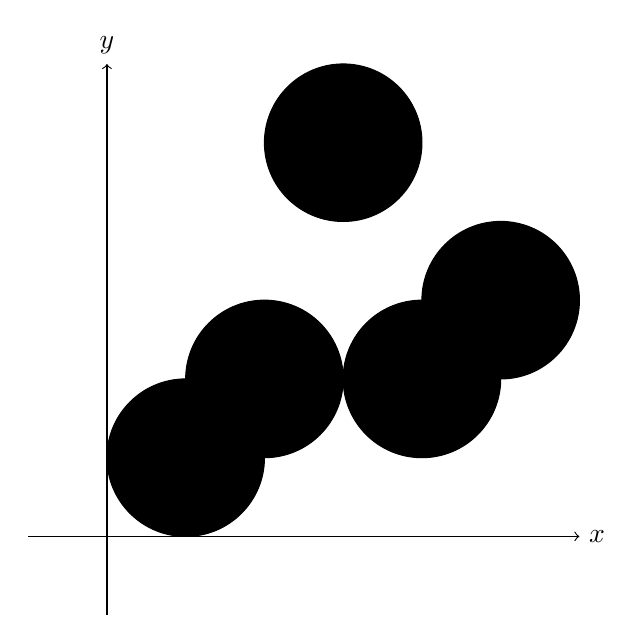
\begin{tikzpicture}
      \draw[->] (-1, 0) -- (6, 0) node[right] {$x$};
      \draw[->] (0, -1) -- (0, 6) node[above] {$y$};
      \foreach \x/\y in {1/1, 2/2, 3/5, 4/2, 5/3} {
         \filldraw (\x, \y) circle (\pointSize) node[below] {$(\x; \y)$};
      }
   \end{tikzpicture}
   \caption{Đồ thị cho ví dụ của $y = f(x)$ được cho ở bảng \ref{tab:ham_so_mot_bien:dinh_nghia:vddths}}
   \label{fig:ham_so_mot_bien:dinh_nghia:vddths}
\end{figure}

Một cách tương tự, chúng ta cũng có thể biểu diễn phương bất hệ thông qua việc vẽ đồ thị chứa các nghiệm của phương bất hệ đó. Có bao nhiêu ẩn số trong phương bất hệ, đồ thị sẽ có bấy nhiêu chiều. Giả sử như bạn đọc cần biểu diễn phương trình $x^2 - 1 = 0$ với $x$ xác định trên tập số thực. Để biểu diễn được phương trình này, trước hết cần phải thực hiện giải nó. Tác giả kì vọng bạn đọc có thể thực hiện được những biến đổi sau:
\begin{align*}
   x^2 - 1 &= 0 \\
   \iff x^2 &= 1 \\
   \iff x &\in \{-1; 1\}.
\end{align*}
Do phương trình chỉ có một ẩn nên chúng ta sẽ chọn trục số một chiều biểu diễn $x$ để thể hiện nghiệm của phương trình này, như hình \ref{fig:ham_so_mot_bien:dinh_nghia:vdgpt}.

\begin{figure}[h]
   \centering
   \begin{tikzpicture}
      \draw[->] (-3, 0) -- (3, 0) node[right] {$x$};
      \foreach \x in {-1, 1} {
         \filldraw[color=colorEmphasisCyan] (\x, 0) circle (\pointSize) node[below] {$(\x)$};
      }
   \end{tikzpicture}
   \caption{Biểu diễn nghiệm của $x^2 - 1 = 0$}
   \label{fig:ham_so_mot_bien:dinh_nghia:vdgpt}
\end{figure}

Về mặt lợi ích của việc sử dụng đồ thị, biểu diễn hình học các đại lượng đại số là một trong những cách hữu hiệu để mở rộng cảm nhận về đối tượng đang nghiên cứu.
      
\exercise Mỗi phần trong bài tập sau bao gồm mối liên hệ giữa $x$ và $y$. Trong mỗi phần, $y$ có phải là hàm của $x$ hay không? Trong trường hợp $y$ là hàm số của $x$, xác định tập xác định và tập giá trị của hàm số đó. Còn trong trường hợp ngược lại, giải thích tại sao $y$ lại không phải là hàm số của $x$.

1.
\begin{tabular}{|c|c|c|c|c|c|}
   \hline
   $x$ & $1$ & $2$ & $3$ & $4$ & $5$ \\
   \hline
   $y$ & $2$ & $3$ & $4$ & $5$ & $6$ \\
   \hline
\end{tabular};

2.
\begin{tabular}{|c|c|c|c|c|c|}
   \hline
   $x$ & $0$ & $-1$ & $1$ & $2$ & $-3$ \\
   \hline
   $y$ & $0$ & $0$ & $0$ & $0$ & $0$ \\
   \hline
\end{tabular};

3.
\begin{tabular}{|c|c|c|c|c|c|}
   \hline
   $x$ & $15$ & $15$ & $16$ & $16$ & $17$ \\
   \hline
   $y$ & $123$ & $134$ & $578$ & $426$ & $348$ \\
   \hline
\end{tabular};

4.
\begin{tabular}{|c|c|c|c|c|c|}
   \hline
   $x$ & $0$ & $-17$ & $3$ & $55$ & $-17$ \\
   \hline
   $y$ & $4586$ & $1024$ & $4586$ & $4586$ & $1024$ \\
   \hline
\end{tabular};

5. $x$ là số chỉ tháng và $y$ là số ngày trong tháng $x$.

\solution

1. $y$ là hàm của $x$ với tập xác định $X = \{1; 2; 3; 4; 5\}$ và tập giá trị $Y = \{2; 3; 4; 5; 6\}$.

2. $y$ là hàm của $x$ với tập xác định $X = \{0; -1; 1; 2; -3\}$ và tập giá trị $Y = \{0\}$.

3. $y$ không phải là hàm của $x$ do khi $x$ có giá trị $15$ thì $y$ có hai giá trị $123$ và $134$.

4. $y$ là hàm của $x$ với tập xác định $X = \{0; -17; 3; 55\}$ và tập giá trị $Y = \{4586; 1024\}$. Lưu ý rằng bảng có cột bị lặp.

5. $y$ không là hàm của $x$ do khi $x = 2$ thì $y$ có hai giá trị $28$ và $29$. Mặc dù cách viết có thể ám chỉ $y=f(x)$ với $f$ là hàm số đại diện cho số ngày trong tháng, nhưng $f$ không phải là hàm số do điều ngoại lệ.

\exercise[ex:ham_so_mot_bien:dinh_nghia:intropt] Vẽ đồ thị của phương trình $\mathcal{P}$, với các định nghĩa được cho. Hàm có tập xác định là bộ số đầu vào cho ở trong bảng. Để ý số ẩn của phương trình để chọn số chiều của đồ thị cho phù hợp.

\begin{enumerate}
   \item
   \begin{tabular}{|c|c|c|c|c|c|c|}
      \hline
      $x$ & $-1$ & $1$ & $-2$ & $2$ & $-3$ & $3$\\
      \hline
      $f(x)$ & $0$ & $0$ & $4$ & $3$ & $7$ & $0$\\
      \hline
   \end{tabular} và $\mathcal{P}: f(x) = 0$;

   \item
   \begin{tabular}{|c|c|c|c|c|c|c|}
      \hline
      $x$ & $-1$ & $1$ & $-2$ & $2$ & $-3$ & $3$\\
      \hline
      $f(x)$ & $0$ & $0$ & $4$ & $3$ & $7$ & $0$\\
      \hline
   \end{tabular} và $\mathcal{P}: f(x) = x^2 - 1$;

   \item
   \begin{tabular}{|c|c|c|c|c|c|c|}
      \hline
      $x$ & $1$ & $2$ & $3$ & $4$ & $5$ & $6$\\
      \hline
      $f(x)$ & $2$ & $3$ & $5$ & $7$ & $11$ & $13$\\
      \hline
      $g(x)$ & $1$ & $3$ & $5$ & $7$ & $9$ & $11$\\
      \hline
   \end{tabular} và $\mathcal{P}: f(x) = g(x)$;

   \item
   \begin{tabular}{|c|c|c|c|c|c|c|}
      \hline
      $x$ & $1$ & $2$ & $3$ & $4$ & $5$ & $6$\\
      \hline
      $f(x)$ & $2$ & $3$ & $5$ & $7$ & $11$ & $13$\\
      \hline
      $g(x)$ & $1$ & $3$ & $5$ & $7$ & $9$ & $11$\\
      \hline
   \end{tabular} và $\mathcal{P}: f(x) = g(y)$;

   \item
   \begin{tabular}{|c|c|c|c|c|c|c|}
      \hline
      $x$ & $1$ & $2$ & $3$ & $4$ & $5$ & $6$\\
      \hline
      $f(x)$ & $2$ & $3$ & $5$ & $7$ & $11$ & $13$\\
      \hline
   \end{tabular} và $\mathcal{P}: f(x) = 2b-1$ với $b \in \mathbb{R}$;

   \item
   \begin{tabular}{|c|c|c|c|c|c|c|}
      \hline
      $x$ & $-1$ & $1$ & $-2$ & $2$ & $-3$ & $3$\\
      \hline
      $f(x)$ & $0$ & $0$ & $4$ & $3$ & $7$ & $0$\\
      \hline
   \end{tabular} và $\mathcal{P}: f(x) = f(2b - 1)$;

   \item 
   \begin{tabular}{|c|c|c|c|c|c|c|}
      \hline
      $x$ & $-1$ & $1$ & $-2$ & $2$ & $-3$ & $3$\\
      \hline
      $f(x)$ & $0$ & $0$ & $4$ & $3$ & $7$ & $0$\\
      \hline
   \end{tabular} và $\mathcal{P}: f(a) + f(b) = f(c)$;
\end{enumerate}

\solution[ex:ham_so_mot_bien:dinh_nghia:intropt]

{
   \begin{minipageindent}{0.48\textwidth}
      \indent 1. $\mathcal{P}$ là phương trình chỉ có một ẩn $x$, do đó đồ thị của $\mathcal{P}$ chỉ là đồ thị một chiều trên một trục số biểu diễn cho $x$.

      Có ba giá trị để $f(x)$ bằng $0$: $x\in \{-1; 1; -3\}$. Chúng ta có đồ thị của $\mathcal{P}$ ở hình \ref{fig:ham_so_mot_bien:dinh_nghia:dtp1}.
   \end{minipageindent}
   \hfill
   \begin{minipageindent}{0.48\textwidth}
      \begin{figure}[H]
         \centering
         \begin{tikzpicture}
            \draw[->] (-2, 0) -- (4, 0) node[right] {$x$};
            \foreach \x in {1, -1, 3} {
               \filldraw[color=colorEmphasisCyan] (\x, 0) circle (\pointSize) node[below] {$(\x)$};
            }
         \end{tikzpicture}
         \caption{Đồ thị phần 1 bài \ref{ex:ham_so_mot_bien:dinh_nghia:intropt}}
         \label{fig:ham_so_mot_bien:dinh_nghia:dtp1}
      \end{figure}
   \end{minipageindent}
}


{
   \begin{minipageindent}{0.48\textwidth}
      2. Tập xác định của $f(x)$ là $\{-1; 1; -2; 2; -3; 3\}$, do đó, để $\mathcal{P}$ thỏa mãn thì $x$ chỉ có thể nhận các giá trị trong vùng tập xác định.

      Kẻ bảng so sánh:
      \begin{table}[H]
         \centering
         \begin{tabular}{|c|c|c|c|c|c|c|}
            \hline
            $x$ & $-1$ & $1$ & $-2$ & $2$ & $-3$ & $3$\\
            \hline
            $f(x)$ & $0$ & $0$ & $4$ & $3$ & $7$ & $0$\\
            \hline
            $x^2-1$ & $0$ & $0$ & $3$ & $3$ & $7$ & $7$\\
            \hline
         \end{tabular}
         \caption{Giá trị của $f(x)$ và $x^2-1$ ứng với $x$}
         \label{tab:ham_so_mot_bien:dinh_nghia:values3}
      \end{table}

      Nhận thấy rằng $\mathcal{P}$ chỉ đúng khi $x\in \{-1; 1; -3; 2\}$ và chúng ta có đồ thị là hình \ref{fig:ham_so_mot_bien:dinh_nghia:dtp2}.
   \end{minipageindent}
   \hfill
   \begin{minipageindent}{0.48\textwidth}
      \begin{figure}[H]
         \centering
         \begin{tikzpicture}
            \draw[->] (-3.5, 0) -- (2.5, 0) node[right] {$x$};
            \foreach \x in {1, -1, -3, 2} {
               \filldraw[color=colorEmphasisCyan] (\x, 0) circle (\pointSize) node[below] {$(\x)$};
            }
         \end{tikzpicture}
         \caption{Đồ thị phần 2 bài \ref{ex:ham_so_mot_bien:dinh_nghia:intropt}}
         \label{fig:ham_so_mot_bien:dinh_nghia:dtp2}
      \end{figure}
   \end{minipageindent}
}

{
   \begin{minipageindent}{0.48\textwidth}
      3. Nhìn vào bảng được cho, có $f(x) = g(x)$ khi và chỉ khi $x\in \{2; 3; 4\}$. Do đó, đồ thị của $\mathcal{P}$ có được như hình \ref{fig:ham_so_mot_bien:dinh_nghia:dtp3}.
   \end{minipageindent}
   \hfill
   \begin{minipageindent}{0.48\textwidth}
      \begin{figure}[H]
         \centering
         \begin{tikzpicture}
            \draw[->] (0, 0) -- (5, 0) node[right] {$x$};
            \foreach \x in {2, 3, 4} {
               \filldraw[color=colorEmphasisCyan] (\x, 0) circle (\pointSize) node[below] {$(\x)$};
            }
         \end{tikzpicture}
         \caption{Đồ thị phần 3 bài \ref{ex:ham_so_mot_bien:dinh_nghia:intropt}}
         \label{fig:ham_so_mot_bien:dinh_nghia:dtp3}
      \end{figure}
   \end{minipageindent}
}

{
   \begin{minipageindent}{0.48\textwidth}
      4. $\mathcal{P}$ là phương trình có hai ẩn $x$ và $y$, do đó đồ thị của $\mathcal{P}$ là một mặt phẳng hai chiều. Coi như trục hoành biểu diễn cho $x$ và trục tung biểu diễn cho $y$. 

      Để có thể vẽ được đồ thị của $\mathcal{P}$, hiển nhiên nhìn ra được rằng cần phải có những điểm $(x;y)$ để hai giá trị $f(x)$ và $g(y)$ bằng nhau. Và để làm được điều đó, trước hết, chúng ta sẽ tìm xem giá trị bằng nhau của $f(x)$ với $g(y)$ này bằng bao nhiêu. Gọi chung giá trị bằng nhau này là $B_n$. Kẻ lại bảng so sánh thành bảng \ref{tab:ham_so_mot_bien:dinh_nghia:bn_values}, với $B_n$ là giá trị đầu ra và $x$, $y$ là giá trị lần lượt đưa vào hai hàm $f$ và $g$ để có giá trị đầu ra đó. Và từ đó, chúng ta có đồ thị của $\mathcal{P}$ là hình \ref{fig:ham_so_mot_bien:dinh_nghia:dtp4}.
   \end{minipageindent}
   \hfill
   \begin{minipageindent}{0.48\textwidth}
      \begin{table}[H]
         \centering
         \begin{tabular}{|c|c|c|c|c|}
            \hline
            $B_n$ & $3$ & $5$ & $7$ & $11$ \\
            \hline
            $x$ & $2$ & $3$ & $4$ & $5$ \\
            \hline
            $y$ & $2$ & $3$ & $4$ & $6$ \\
            \hline 
         \end{tabular}
         \caption{Giá trị của $x$ và $y$ ứng với $B_n$}
         \label{tab:ham_so_mot_bien:dinh_nghia:bn_values}
      \end{table}
   \end{minipageindent}
}

\begin{figure}[H]
   \centering
   \begin{tikzpicture}
      \draw[->] (0, 0) -- (3.5, 0) node[right] {$x$};
      \draw[->] (0, 0) -- (0, 3.5) node[above] {$y$};
      \filldraw[color=colorEmphasisCyan] (1, 1) circle (\pointSize) node[right] {$(2; 2)$};
      \filldraw[color=colorEmphasisCyan] (1.5, 1.5) circle (\pointSize) node[right] {$(3; 3)$};
      \filldraw[color=colorEmphasisCyan] (2.5, 3) circle (\pointSize) node[right] {$(5; 6)$};
      \filldraw[color=colorEmphasisCyan] (2, 2) circle (\pointSize) node[right] {$(4; 4)$};
   \end{tikzpicture}
   \caption{Đồ thị phần 4 bài \ref{ex:ham_so_mot_bien:dinh_nghia:intropt}}
   \label{fig:ham_so_mot_bien:dinh_nghia:dtp4}
\end{figure}

{
   \begin{minipageindent}{0.48\textwidth}
      5. $\mathcal{P}$ là phương trình có hai ẩn $x$ và $b$, do đó đồ thị của $\mathcal{P}$ là một mặt phẳng hai chiều. Coi như trục hoành biểu diễn cho $x$ và trục tung biểu diễn cho $b$.

      Tính giá trị của $b$ từ $f(x)$:
      \begin{align*}
         f(x) &= 2b - 1 \\
         \iff b &= \frac{f(x) + 1}{2}.
      \end{align*}
   \end{minipageindent}
   \hfill
   \begin{minipageindent}{0.48\textwidth}
      \begin{table}[H]
         \centering
         \begin{tabular}{|c|c|c|c|c|c|c|}
            \hline
            $x$ & $1$ & $2$ & $3$ & $4$ & $5$ & $6$\\
            \hline
            $f(x)$ & $2$ & $3$ & $5$ & $7$ & $11$ & $13$\\
            \hline
            $b$ & $\frac{3}{2}$ & $\frac{5}{2}$ & $3$ & $4$ & $6$ & $7$\\
            \hline
         \end{tabular}
         \caption{Giá trị của $b$ ứng với $x$}
         \label{tab:ham_so_mot_bien:dinh_nghia:b_values6}
      \end{table}
   \end{minipageindent}
}
Từ đây, chúng ta có thể thêm giá trị của $b$ vào bảng được cho thành bảng \ref{tab:ham_so_mot_bien:dinh_nghia:b_values6}. 

Qua bảng đó, vẽ được đồ thị của $\mathcal{P}$ như hình \ref{fig:ham_so_mot_bien:dinh_nghia:dtp5}.


\begin{figure}[H]
   \centering
   \begin{tikzpicture}
      \draw[->] (0, 0) -- (4, 0) node[right] {$x$};
      \draw[->] (0, 0) -- (0, 4) node[above] {$b$};
      \filldraw[color=colorEmphasisCyan] (0.5, 0.75) circle (\pointSize) node[below] {$\left(1; \frac{3}{2}\right)$};
      \filldraw[color=colorEmphasisCyan] (1, 1.25) circle (\pointSize) node[below] {$\left(2; \frac{5}{2}\right)$};
      \filldraw[color=colorEmphasisCyan] (1.5, 1.5) circle (\pointSize) node[right] {$(3; 3)$};
      \filldraw[color=colorEmphasisCyan] (2, 2) circle (\pointSize) node[right] {$(4; 4)$};
      \filldraw[color=colorEmphasisCyan] (2.5, 3) circle (\pointSize) node[right] {$(5; 6)$};
      \filldraw[color=colorEmphasisCyan] (3, 3.5) circle (\pointSize) node[right] {$(6; 7)$};
   \end{tikzpicture}
   \caption{Đồ thị phần 5 bài \ref{ex:ham_so_mot_bien:dinh_nghia:intropt}}
   \label{fig:ham_so_mot_bien:dinh_nghia:dtp5}
\end{figure}

{
   \begin{minipageindent}{0.48\textwidth}
      6. Nhìn vào bảng định nghĩa được cho, $f(x)$ có thể nhận các giá trị là $\{0; 3; 4; 7\}$.

      \textcolor{colorEmphasis}{Trường hợp một}: Khi $f(x) \neq 0$, chỉ có một giá trị đầu vào cho $f$ sao cho $f(x)$ đạt được giá trị đầu ra. Ví dụ, chỉ có đầu vào $x = 2$ mới có $f(x) = 3$. Do đó, khi $f(x) \neq 0$, $x = 2b-1$. Biến đổi đại số cơ bản để có $b = \frac{x + 1}{2}$. Lập bảng \ref{tab:ham_so_mot_bien:dinh_nghia:b_values7} để thấy được mối quan hệ giữa $x$ và $b$.

   \end{minipageindent}
   \hfill
   \begin{minipageindent}{0.48\textwidth}
      \begin{table}[H]
         \centering
         \begin{tabular}{|c|c|c|c|}
            \hline
            $x$ & $-2$ & $2$ & $-3$\\
            \hline
            $b = \frac{x+1}{2}$ & $-\frac{3}{2}$ & $2$ & $-1$\\
            \hline
         \end{tabular}
         \caption{Giá trị của cặp $(x; b)$ với $f(x) \neq 0$}
         \label{tab:ham_so_mot_bien:dinh_nghia:b_values7}
      \end{table}
   \end{minipageindent}
}

\textcolor{colorEmphasisCyan}{Trường hợp hai}: Khi $f(x) = 0$, $x$ và $2b-1$ có thể nhận bất cứ giá trị nào trong tập $\{-1; 1; -3\}$. Từ đó, có thể chọn $x \in \{-1; 1; 3\}$ và giải đại số để chọn $b \in \left\{\frac{-1+1}{2}; \frac{1+1}{2}; \frac{3+1}{2}\right\} = \{0; 1; 2\}$. Các cặp $(x; b)$ thỏa mãn là $(x; b)$ $\in$ $\{\left(-1; 0\right); \left(-1; 1\right); \left(-1; 2\right); \left(1; 0\right); \left(1; 1\right); \left(1; 2\right); \left(-3; 0\right); \left(-3; 1\right); \left(-3; 2\right)\}$.

Cuối cùng, kết hợp hai trường hợp, chúng ta có đồ thị cho $\mathcal{P}$:
\begin{figure}[H]
   \centering
   \begin{tikzpicture}
      \draw[->] (-4, 0) -- (3, 0) node[right] {$x$};
      \draw[->] (0, -2.5) -- (0, 2.5) node[above] {$b$};
      
      % Vẽ phần f(x) khác 0
      \filldraw[color=colorEmphasis] (-2, -1.5) circle (\pointSize) node[below] {$\left(-2; -\frac{3}{2}\right)$};
      \filldraw[color=colorEmphasis] (2, 2) circle (\pointSize) node[below] {$\left(2; 2\right)$};
      \filldraw[color=colorEmphasis] (-3, -1) circle (\pointSize) node[below] {$\left(-3; -1\right)$};
      
      \filldraw[color=colorEmphasisCyan] (-1, 0) circle (\pointSize) node[below] {$\left(-1; 0\right)$};
      \filldraw[color=colorEmphasisCyan] (1, 0) circle (\pointSize) node[below] {$\left(1; 0\right)$};
      \filldraw[color=colorEmphasisCyan] (-3, 0) circle (\pointSize) node[below] {$\left(-3; 0\right)$};
      
      \filldraw[color=colorEmphasisCyan] (-1, 1) circle (\pointSize) node[below] {$\left(-1; 1\right)$};
      \filldraw[color=colorEmphasisCyan] (1, 1) circle (\pointSize) node[below] {$\left(1; 1\right)$};
      \filldraw[color=colorEmphasisCyan] (-3, 1) circle (\pointSize) node[below] {$\left(-3; 1\right)$};
      
      \filldraw[color=colorEmphasisCyan] (-1, 2) circle (\pointSize) node[below] {$\left(-1; 2\right)$};
      \filldraw[color=colorEmphasisCyan] (1, 2) circle (\pointSize) node[below] {$\left(1; 2\right)$};
      \filldraw[color=colorEmphasisCyan] (-3, 2) circle (\pointSize) node[below] {$\left(-3; 2\right)$};
   \end{tikzpicture}
   \caption{Đồ thị phần 6 bài \ref{ex:ham_so_mot_bien:dinh_nghia:intropt}}
   \label{fig:ham_so_mot_bien:dinh_nghia:dtp7}
\end{figure}

7. $\mathcal{P}$ là phương trình có ba ẩn $a$, $b$ và $c$, do đó đồ thị của $\mathcal{P}$ là một không gian ba chiều với các trục hoành, trục tung và trục cao tương ứng là $a$, $b$ và $c$.

Theo $\mathcal{P}$, chúng ta cần phải chọn ba số trong tập giá trị của $f$ để hai trong ba số có tổng bằng số còn lại. Từ bảng, nhận thấy rằng, chỉ có thể có hai tổng $4 + 3 = 7$ và $0 + 0 = 0$.

Chúng ta cần tìm tất cả các bộ ba $(a, b, c)$ thỏa mãn $f(a) + f(b) = f(c)$. Xét hai trường hợp sau:

\textcolor{colorEmphasis}{Trường hợp một}: Tổng hai số khác 0. Để $f(a) + f(b) = f(c)$, chỉ có thể xảy ra khi $3 + 4 = 7$. Do đó, $(f(a); f(b); f(c))$ phải là $(3; 4; 7)$ hoặc $(4; 3; 7)$. Tra ngược lại bảng giá trị, chúng ta có hai nghiệm:
   \begin{itemize}
      \item $f(a)=3, f(b)=4 \implies a=2, b=-2$. Và
      \item $f(a)=4, f(b)=3 \implies a=-2, b=2$.
   \end{itemize}

Chỉ có $f(-3) = 7$ nên $c = -3$.

\textcolor{colorEmphasisCyan}{Trường hợp hai}: Tất cả bằng 0. Khi $f(a) = f(b) = f(c) = 0$, từ bảng định nghĩa, $f(x)=0$ khi $x \in \{-3; -1; 1\}$. Do đó, $a, b, c$ có thể nhận bất kỳ giá trị nào trong tập $\{-3; -1; 1\}$. Có tổng cộng $3^3 = 27$ bộ ba thỏa mãn trong trường hợp này.

Kết hợp hai trường hợp, đồ thị của $\mathcal{P}$ sẽ gồm 29 điểm trong không gian 3 chiều (2 điểm từ trường hợp 1 và 27 điểm từ trường hợp 2), được biểu diễn trong hình \ref{fig:ham_so_mot_bien:dinh_nghia:dtp8}.

\begin{figure}[H]
   \centering
   \tdplotsetmaincoords{80}{30}
   \begin{tikzpicture}[tdplot_main_coords]
      \draw[->] (-5, 0, 0) -- (2, 0, 0) node[right] {$a$};
      \draw[->] (0, -5, 0) -- (0, 4, 0) node[above] {$b$};
      \draw[->] (0, 0, -4) -- (0, 0, 2) node[above] {$c$};
      \filldraw[color=colorEmphasis] (2, -2, -3) circle (\pointSize) node[font=\scriptsize, anchor=north] {$\left(2; -2; -3\right)$};  
      \filldraw[color=colorEmphasis] (-2, 2, -3) circle (\pointSize) node[font=\scriptsize, anchor=south] {$\left(-2; 2; -3\right)$};  
      \foreach \x/\y/\z in {
         -3/-3/-3, -3/-3/-1, -3/-3/1, 
         -3/-1/-3, -3/-1/-1, -3/-1/1, -3/1/-3, -3/1/-1, -3/1/1,
         -1/-3/-3, -1/-3/-1, -1/-3/1, -1/-1/-3, -1/-1/-1, -1/-1/1,
         -1/1/-3, -1/1/-1, -1/1/1, 1/-3/-3, 1/-3/-1, 1/-3/1,
         1/-1/-3, 1/-1/-1, 1/-1/1, 1/1/-3, 1/1/-1, 1/1/1
      } {
         \filldraw[color=colorEmphasisCyan] (\x, \y, \z) circle (\pointSize);
         \node[font=\scriptsize, anchor=east, color=colorEmphasisCyan] at (\x, \y, \z) {$\left(\x; \y; \z\right)$};
      }
   \end{tikzpicture}
   \caption{Đồ thị phần 7 bài \ref{ex:ham_so_mot_bien:dinh_nghia:intropt}}
   \label{fig:ham_so_mot_bien:dinh_nghia:dtp8}
\end{figure}

\exercise[ex:ham_so_mot_bien:dinh_nghia:bpt1] Vẽ đồ thị của bất phương trình $\mathcal{P}$, với các định nghĩa đã cho. Hàm có tập xác định là bộ số đầu vào cho ở trong bảng.
\begin{enumerate}
   \item 
   \begin{tabular}{|c|c|c|c|c|c|c|}
      \hline
      $x$ & $0$ & $1$ & $2$ & $3$ & $4$ & $5$ \\
      \hline
      $f(x)$ & $-1$ & $-3$ & $-4$ & $-2$ & $-1$ & $-3$\\
      \hline
   \end{tabular} và $\mathcal{P}:f(x) \neq -3$;

   \item 
   \begin{tabular}{|c|c|c|c|c|c|c|}
      \hline
      $x$ & $-10$ & $-8$ & $-2$ & $2$ & $8$ & $10$ \\
      \hline
      $\alpha(x)$ & $4$ & $8$ & $0$ & $1$ & $6$ & $8$\\
      \hline
   \end{tabular} và $\mathcal{P}:\alpha(x) < 0$;

   \item 
   \begin{tabular}{|c|c|c|c|c|c|c|}
      \hline
      $x$ & $0$ & $6$ & $2$ & $-7$ & $-6$ & $3$ \\
      \hline
      $\beta(x)$ & $4$ & $7$ & $10$ & $3$ & $10$ & $9$\\
      \hline
   \end{tabular} và $\mathcal{P}:\beta(x) > x$;

   \item 
   \begin{tabular}{|c|c|c|c|c|c|c|}
      \hline
      $x$ & $-10$ & $-8$ & $-2$ & $2$ & $8$ & $10$ \\
      \hline
      $\alpha(x)$ & $4$ & $8$ & $0$ & $1$ & $6$ & $8$\\
      \hline
   \end{tabular},
   \begin{tabular}{|c|c|c|c|c|c|c|}
      \hline
      $x$ & $0$ & $6$ & $2$ & $-7$ & $-6$ & $3$ \\
      \hline
      $\beta(x)$ & $4$ & $7$ & $10$ & $3$ & $10$ & $9$\\
      \hline
   \end{tabular}, và $\mathcal{P}:\alpha(x) \geq 2\beta(y)$.
\end{enumerate}

\solution[ex:ham_so_mot_bien:dinh_nghia:bpt1]

{
   \begin{minipageindent}{0.48\textwidth}
      1. Phần này tương đối đơn giản. Kiểm tra trên bảng, chúng ta thấy $f(x) = -3$ khi $x \in \{2; 5\}$. Thêm vào đó, tập xác định của $f$ là $\{0; 1; 2; 3; 4; 5\}$. Do đó, $f(x) \neq -3$ khi $x \in \{0; 1; 3; 4\}$. 

      Đồ thị của $\mathcal{P}$ là hình \ref{fig:ham_so_mot_bien:dinh_nghia:bpt1} ở bên.
   \end{minipageindent}
   \begin{minipageindent}{0.48\textwidth}
      \begin{figure}[H]
         \centering
         \begin{tikzpicture}
            \draw[->] (-1, 0) -- (5, 0) node[right] {$x$};
            \foreach \x in {0, 1, 3, 4} {
               \filldraw[color=colorEmphasisCyan] (\x, 0) circle (\pointSize) node[below] {$\left(\x\right)$};
            }
         \end{tikzpicture}
         \caption{Đồ thị phần 1 bài \ref{ex:ham_so_mot_bien:dinh_nghia:bpt1}}
         \label{fig:ham_so_mot_bien:dinh_nghia:bpt1}
      \end{figure}
   \end{minipageindent}
}

{
   \begin{minipageindent}{0.48\textwidth}
      2. Tra bảng trực tiếp, các giá trị $\alpha(x)$ không bao giờ nhỏ hơn $0$. Chúng ta không xét giá trị $x$ ngoài bảng do không thuộc tập xác định của hàm $\alpha$. Do đó, $\alpha(x) < 0$ là bất phương trình vô nghiệm.

      Và qua đó, vẽ được đồ thị của $\mathcal{P}$ là trục không đánh dấu như hình \ref{fig:ham_so_mot_bien:dinh_nghia:bpt2}.
   \end{minipageindent}
   \begin{minipageindent}{0.48\textwidth}
      \begin{figure}[H]
         \centering
         \begin{tikzpicture}
            \draw[->] (-1, 0) -- (5, 0) node[right] {$x$};
         \end{tikzpicture}
         \caption{Đồ thị phần 2 bài \ref{ex:ham_so_mot_bien:dinh_nghia:bpt1}}
         \label{fig:ham_so_mot_bien:dinh_nghia:bpt2}
      \end{figure}
   \end{minipageindent}
}

3. Xét trên tập xác định của $\beta$, chúng ta có $\beta(x) > x$ với mọi $x$ nằm trên bảng được cho. Một cách đơn giản, chúng ta có đồ thị là hình \ref{fig:ham_so_mot_bien:dinh_nghia:bpt3}.

\begin{figure}[H]
   \centering
   \begin{tikzpicture}
      \draw[->] (-8, 0) -- (8, 0) node[right] {$x$};
      \foreach \x in {0, 6, 2, -7, -6, 3} {
         \filldraw[color=colorEmphasisCyan] (\x, 0) circle (\pointSize) node[below] {$\left(\x\right)$};
      }
   \end{tikzpicture}
   \caption{Đồ thị phần 3 bài \ref{ex:ham_so_mot_bien:dinh_nghia:bpt1}}
   \label{fig:ham_so_mot_bien:dinh_nghia:bpt3}
\end{figure}

4. Chúng ta có thể kiểm tra trực tiếp $36$ cặp $(x; y)$ và sau đó vẽ đồ thị. Sau đây, tác giả sẽ chỉ những góc nhìn để có thể giảm số trường hợp cần kiểm tra.

Để ý rằng, giá trị lớn nhất có thể của $\alpha(x)$ là $8$. Mặt khác, để $\mathcal{P}$ thỏa mãn thì
\begin{align*}
   \alpha(x) &\geq 2\beta(y) \\
   \iff \beta(y) &\leq \frac{\alpha(x)}{2}. \\
\end{align*}
Qua đó, giá trị lớn nhất có thể của $\beta(y)$ là $4$. Theo bảng định nghĩa, $\beta(y)$ chỉ có thể nhận hai giá trị là $3$ hoặc $4$. 

\textcolor{colorEmphasisCyan}{Trường hợp một}: $\beta(y) = 3 \iff y = -7$. Khi này, để $\alpha(x) \geq 2\beta(x)$ hay $\alpha(x) \geq 6$ thì $\alpha(x)$ có thể nhận giá trị $8$ hoặc $6$. Do đó,
\begin{align*}
   &\alpha(x) = 6 \implies x = 8;\\
   &\alpha(x) = 8 \implies x \in \{-8; 10\}.
\end{align*}

\textcolor{colorEmphasis}{Trường hợp hai}: $\beta(y) = 4 \iff y = 0$. Khi này, để $\alpha(x) \geq 8$ thì $\alpha(x)$ chỉ có thể nhận bằng $8$. Do đó, $x \in \{-8; 10\}$.

Từ đây, chúng ta có đồ thị \ref{fig:ham_so_mot_bien:dinh_nghia:bpt4}.

\begin{figure}[H]
   \centering
   \begin{tikzpicture}
      \draw[->] (-4, 0) -- (4, 0) node[right] {$x$};
      \draw[->] (0, -3) -- (0, 0) node[above] {$y$};
      \foreach \x/\y/\pos in {8/-7/above, -8/-7/below, 10/-7/below} {
         \filldraw[color=colorEmphasisCyan] (\x/3, \y/3) circle (\pointSize) node [\pos] {$\left(\x; \y\right)$};
      }
      \foreach \x/\y/\pos in {-8/0/below, 10/0/below} {
         \filldraw[color=colorEmphasis] (\x/3, \y/3) circle (\pointSize) node [\pos] {$\left(\x; \y\right)$};
      }
   \end{tikzpicture}
   \caption{Đồ thị phần 4 bài \ref{ex:ham_so_mot_bien:dinh_nghia:bpt1}}
   \label{fig:ham_so_mot_bien:dinh_nghia:bpt4}
\end{figure}

\exercise[ex:ham_so_mot_bien:dinh_nghia:hpt1] Vẽ đồ thị của hệ phương trình $\mathcal{P}$, với các định nghĩa đã cho. Hàm có tập xác định là bộ số đầu vào cho ở trong bảng.
\begin{enumerate}
   \item 
   \begin{tabular}{|c|c|c|c|c|c|c|}
      \hline
      $x$ & $0$ & $1$ & $2$ & $3$ & $4$ & $5$ \\
      \hline
      $f(x)$ & $-1$ & $-1$ & $-1$ & $-2$ & $-3$ & $-3$\\
      \hline
   \end{tabular},
   \begin{tabular}{|c|c|c|c|c|c|c|}
      \hline
      $y$ & $0$ & $-2$ & $4$ & $-6$ & $8$ & $-10$\\
      \hline
      $g(y)$ & $-1$ & $-2$ & $-3$ & $-7$ & $-8$ & $-9$\\
      \hline
   \end{tabular},

   \noindent\begin{tabular}{|c|c|c|c|c|c|c|}
      \hline
      $z$ & $-1$ & $1$ & $-2$ & $0$ & $-4$ & $4$\\
      \hline
      $h(z)$ & $2$ & $1$ & $0$ & $-1$ & $-2$ & $-3$\\
      \hline
   \end{tabular} và $\mathcal{P}:f(x) = g(x) = h(x)$;

   \item
   \begin{tabular}{|c|c|c|c|c|c|c|}
      \hline
      $x$ & $0$ & $1$ & $2$ & $3$ & $4$ & $5$ \\
      \hline
      $f(x)$ & $-1$ & $-1$ & $-1$ & $-2$ & $-3$ & $-3$\\
      \hline
   \end{tabular},
   \begin{tabular}{|c|c|c|c|c|c|c|}
      \hline
      $y$ & $0$ & $-2$ & $4$ & $-6$ & $8$ & $-10$\\
      \hline
      $g(y)$ & $-1$ & $-2$ & $-3$ & $-7$ & $-8$ & $-9$\\
      \hline
   \end{tabular},

   \noindent\begin{tabular}{|c|c|c|c|c|c|c|}
      \hline
      $z$ & $-1$ & $1$ & $-2$ & $0$ & $-4$ & $4$\\
      \hline
      $h(z)$ & $2$ & $1$ & $0$ & $-1$ & $-2$ & $-3$\\
      \hline
   \end{tabular} và $\mathcal{P}:f(a) = g(b) = h(c)$;

   \item
   \begin{tabular}{|c|c|c|c|c|c|c|}
      \hline
      $x$ & $0$ & $1$ & $2$ & $3$ & $4$ & $5$ \\
      \hline
      $f(x)$ & $-1$ & $-1$ & $-1$ & $-2$ & $-3$ & $-3$\\
      \hline
   \end{tabular},
   \begin{tabular}{|c|c|c|c|c|c|c|}
      \hline
      $y$ & $0$ & $-2$ & $4$ & $-6$ & $8$ & $-10$\\
      \hline
      $g(y)$ & $-1$ & $-2$ & $-3$ & $-7$ & $-8$ & $-9$\\
      \hline
   \end{tabular},

   \noindent\begin{tabular}{|c|c|c|c|c|c|c|}
      \hline
      $z$ & $-1$ & $1$ & $-2$ & $0$ & $-4$ & $4$\\
      \hline
      $h(z)$ & $2$ & $1$ & $0$ & $-1$ & $-2$ & $-3$\\
      \hline
   \end{tabular} và $\mathcal{P}:\begin{cases}f(o) = g(p)\\f(p + 1) = h(q)\end{cases}$.

   \item
   \begin{tabular}{|c|c|c|c|c|c|c|}
      \hline
      $x$ & $0$ & $1$ & $2$ & $3$ & $4$ & $5$ \\
      \hline
      $f(x)$ & $-1$ & $-1$ & $-1$ & $-2$ & $-3$ & $-3$\\
      \hline
   \end{tabular},
   \begin{tabular}{|c|c|c|c|c|c|c|}
      \hline
      $y$ & $0$ & $-2$ & $4$ & $-6$ & $8$ & $-10$\\
      \hline
      $g(y)$ & $-1$ & $-2$ & $-3$ & $-7$ & $-8$ & $-9$\\
      \hline
   \end{tabular},

   \noindent\begin{tabular}{|c|c|c|c|c|c|c|}
      \hline
      $z$ & $-1$ & $1$ & $-2$ & $0$ & $-4$ & $4$\\
      \hline
      $h(z)$ & $2$ & $1$ & $0$ & $-1$ & $-2$ & $-3$\\
      \hline
   \end{tabular} và $\mathcal{P}:\begin{cases}f(m) = n\\g(n) = h(w)\end{cases}$.
\end{enumerate}

\solution[ex:ham_so_mot_bien:dinh_nghia:hpt1]

1. Giá trị đầu vào để $f, g, h$ đều có cùng một đầu ra là $x\in\{0;4\}$. Vậy, chúng ta có đồ thị như hình \ref{fig:hpt11}.

\begin{figure}[H]
   \centering
   \begin{tikzpicture}
      \draw[->] (-1, 0) -- (5, 0) node[right] {$x$};
      \filldraw[color=colorEmphasisCyan] (0, 0) circle (\pointSize) node[below] {$(0)$};
      \filldraw[color=colorEmphasisCyan] (4, 0) circle (\pointSize) node[below] {$(4)$};
   \end{tikzpicture}
   \caption{Đồ thị phần 1 bài \ref{ex:ham_so_mot_bien:dinh_nghia:hpt1}}
   \label{fig:hpt11}
\end{figure}

2. Trước hết, cần tìm những giá trị chung trong tập giá trị của $f, g, h$. Nhận thấy rằng, có $-1, -2$ và $-3$ là những giá trị chung trong đó. 
\begin{itemize}
   \item Với đầu ra là $-1$, chúng ta có $f(a) = g(b) = h(c) = -1$. Từ đó, chúng ta có $a \in \{0; 1; 2\}$ và $b = c = 0$.
   \item Trong trường hợp kết quả của hàm là $-2$, $f(a) = g(b) = h(c) = -2$. Từ đó, bộ ba $\left(a; b; c\right)$ có giá trị là $(3; -2; -4)$.
   \item Trong trường hợp kết quả của hàm là $-3$, $f(a) = g(b) = h(c) = -3$. Từ đó, $\left(a; b; c\right)$ $\in \left\{\left(4; 4; 4\right); \left(5; 4; 4\right)\right\}$.
\end{itemize}
Kết hợp ba trường hợp, xây dựng không gian tọa độ, chúng ta có hình \ref{fig:hpt12}.

\begin{figure}[H]
   \centering
   \tdplotsetmaincoords{80}{-10}
   \begin{tikzpicture}[tdplot_main_coords]
      \draw[->] (-1.5, 0, 0) -- (3, 0, 0) node[right] {$a$};
      \draw[->] (0, -1, 0) -- (0, 2.5, 0) node[above] {$b$};
      \draw[->] (0, 0, -2.5) -- (0, 0, 2.5) node[above] {$c$};
      \foreach \x/\y/\z/\pos in {
         0/0/0/below left,
         1/0/0/above,
         2/0/0/below} {
            \filldraw[color=colorEmphasisCyan] ({\x/2}, {\y/2}, {\z/2}) circle (\pointSize) node[\pos] {$\left(\x; \y; \z\right)$};
      }
      \filldraw[color=colorEmphasis] (1.5, -1, -2) circle (\pointSize) node[above] {$\left(3; -2; -4\right)$};
      \foreach \x/\y/\z/\pos in {
         4/4/4/above,
         5/4/4/below} {
            \filldraw[color=colorEmphasisGreen] ({\x/2}, {\y/2}, {\z/2}) circle (\pointSize) node[\pos] {$\left(\x; \y; \z\right)$};
      };
   \end{tikzpicture}
   \caption{Đồ thị phần 2 bài \ref{ex:ham_so_mot_bien:dinh_nghia:hpt1}}
   \label{fig:hpt12}
\end{figure}

3. Để $f$ và $g$ nhận cùng một giá trị thì giá trị đầu ra đó, theo bảng định nghĩa được cho, kết quả mà hàm trả ra phải là $-1$, $-2$ hoặc $-3$.
\begin{itemize}
   \item Tại $f(o) = g(p) = -1$, $o \in \{0; 1; 2\}$ và $p = 0$. Từ đó, $f(p + 1) = f(1) = -1$. Khi này, $h(q) = -1 \iff q = 0$.
   \item Tại $f(o) = g(p) = -2$, sau khi tra bảng, chúng ta thấy được rằng $\begin{cases}o = 3\\p = -2\end{cases}$; suy ra $f(p + 1) = f(-1)$, Tuy nhiên, $-1$ không thuộc tập xác định của $f$. Vậy, chúng ta sẽ loại trường hợp này.
   \item Tại $f(o) = g(p) = -3$, $o \in \{4; 5\}$ và $p = 4$. Từ đó, $f(p + 1) = f(5) = -3$. Khi này, $h(q) = -3 \iff q = 4$.
\end{itemize}
Cuối cùng, vẽ đồ thị để được hình \ref{fig:hpt13}.

\begin{figure}[H]
   \tdplotsetmaincoords{80}{-10}
   \centering
   \fbox{
      \begin{tikzpicture}[tdplot_main_coords]
         \draw[->] (-1, 0, 0) -- (3, 0, 0) node[right] {$o$};
         \draw[->] (0, -1, 0) -- (0, 2.5, 0) node[above] {$p$};
         \draw[->] (0, 0, -1) -- (0, 0, 2.5) node[above] {$q$};
         \foreach \x/\y/\z/\pos in {
            0/0/0/below left,
            1/0/0/above,
            2/0/0/below} {
               \filldraw[color=colorEmphasisCyan] ({\x/2}, {\y/2}, {\z/2}) circle (\pointSize) node[\pos] {$\left(\x; \y; \z\right)$};
         }
         \foreach \x/\y/\z/\pos in {
            4/4/4/above,
            5/4/4/below} {
               \filldraw[color=colorEmphasisGreen] ({\x/2}, {\y/2}, {\z/2}) circle (\pointSize) node[\pos] {$\left(\x; \y; \z\right)$};
         };
      \end{tikzpicture}
   }
   \caption{Đồ thị phần 3 bài \ref{ex:ham_so_mot_bien:dinh_nghia:hpt1}}
   \label{fig:hpt13}
\end{figure}

4. Theo đề, chúng ta cần tìm những bộ $(m;n;w)$ thỏa mãn $\mathcal{P}$, trong đó có $g(n) = h(w)$. Cho nên, $n$ phải thuộc tập xác định của $g$. Nhìn vào bảng, tập xác định đó là $\{0; -2; 4; -6; 8; -10\}$. Tuy nhiên, cũng có $f(m) = n$, cho nên $n$ vừa phải thuộc tập giá trị của $f$, hay $n \in \{-1; -2; -3\}$. Lấy giao của hai tập đó, chúng ta có $n = -2$. Từ đó, giải $f(m) = -2$ để có $m = 3$. Thêm vào đó, $h(w) = g(-2) = -2 \iff w = -4$.

Bộ số duy nhất thỏa mãn hệ phương trình $\mathcal{P}$ là $\left(m; n; w\right) = \left(3; -2; -4\right)$. Đồ thị của $\mathcal{P}$ là hình \ref{fig:hpt14}.

\begin{figure}[H]
   \tdplotsetmaincoords{80}{20}
   \centering
   \fbox{
      \begin{tikzpicture}[tdplot_main_coords]
         \draw[->] (-0.5, 0, 0) -- (2, 0, 0) node[right] {$m$};
         \draw[->] (0, -1.5, 0) -- (0, 0.5, 0) node[above] {$n$};
         \draw[->] (0, 0, -2.5) -- (0, 0, 0.5) node[above] {$w$};
         \filldraw[color=colorEmphasisCyan] (1.5, -1, -2) circle (\pointSize ) node[above] {$\left(3; -2; -4\right)$};
      \end{tikzpicture}
   }
   \caption{Đồ thị phần 4 bài \ref{ex:ham_so_mot_bien:dinh_nghia:hpt1}}
   \label{fig:hpt14}
\end{figure}
% \subsection{Kí hiệu tổng và tích của nhiều số}

\ % Lùi đầu dòng

Cho hàm số $f(x)$. Khi cho $x$ là số nguyên chạy từ $a$ đến $b$ (thông thường $a \le b$), chúng ta có tổng của các giá trị $f(x)$ được viết rút gọn là
$$
\defMath{\sum_{x=a}^{b} \left(f(x)\right) = f(a) + f(a + 1) + \cdots + f(b)}.
$$

Ví dụ, nếu cho $f(x) = 3x - 7$, thì
\begin{align*}
   \sum_{x = -1}^3 \left(f(x)\right) &= f(-1) + f(0) + f(1) + f(2) + f(3) \\
   &= \left(3(-1) - 7\right) + \left(3(0) - 7\right) + \left(3(1) - 7\right) + \left(3(2) - 7\right) + \left(3(3) - 7\right) \\
   &= -20.
\end{align*}

Đối với tích của các giá trị $f(x)$, chúng ta có
$$
\defMath{\prod_{x=a}^{b} \left(f(x)\right) = f(a) \times f(a + 1) \times \cdots \times f(b)}.
$$

Ví dụ, cùng với $f(x) = 3x - 7$, chúng ta có
\begin{align*}
   \prod_{x = -1}^3 \left(f(x)\right) &= f(-1) \times f(0) \times f(1) \times f(2) \times f(3) \\
   &= \left(3(-1) - 7\right) \times \left(3(0) - 7\right) \times \left(3(1) - 7\right) \times \left(3(2) - 7\right) \times \left(3(3) - 7\right) \\
   &= 560.
\end{align*}

Mở rộng kí hiệu, nếu chúng ta có cần tính tổng hay tích vào hàm phụ thuộc vào các giá trị $x$ thỏa mãn điều kiện $P$ nào đó, thì chúng ta có thể viết
$$
\defMath{\sum_{P} \left(f(x)\right) \text{ và }\prod_{P} \left(f(x)\right)}.
$$

$P$ có thể được viết theo nhiều kiểu khác nhau, miễn hiểu là được. Ví dụ, thay vì tính tổng và tích của $f(x)$ khi $x$ thay đổi từ $-1$ đến $3$, chúng ta có thể tính tổng và tích của $f(x)$ với $x$ là các số nguyên tố lớn hơn $10$ và nhỏ hơn $20$. Khi đó,

{
   \begin{minipageindent}{0.48\textwidth}
      \begin{align*}
         &\sum\limits_{x \text{ là số nguyên tố lớn hơn } 10 \text{ và nhỏ hơn } 20} \left(f(x)\right) \\
         = &f(11) + f(13) + f(17) + f(19) \\
         = &152\text{, và}
      \end{align*}
   \end{minipageindent}
   \hfill
   \begin{minipageindent}{0.48\textwidth}
      \begin{align*}
         &\prod\limits_{x \text{ là số nguyên tố lớn hơn } 10 \text{ và nhỏ hơn } 20} \left(f(x)\right) \\
         = &f(11) \times f(13) \times f(17) \times f(19) \\
         = &1830400.
      \end{align*}
   \end{minipageindent}
}

% \subsection{Hàm đa thức}

\ % Lùi đầu dòng

Hàm \defText{đa thức} thông thường được biểu diễn dưới dạng tổng của các đơn thức $$\defMath{f(x)=P_n(x)=\sum_{i = 0}^n \left(a_i x^i\right) = a_nx^n + a_{n-1}x^{n-1} + \cdots + a_1x + a_0}$$ với $n$ là một số nguyên không âm, $a_i$ là các số thực, gọi là các \defText{hệ số}, với mọi $i$ nguyên nằm trong đoạn $[0, n]$ và $a_n \neq 0$. Khi này, $n$ được gọi là \defText{bậc} của đa thức\label{def:ham_so_mot_bien:da_thuc:da_thuc}. Mọi giá trị $x \in \mathbb{R}$ đều thuộc tập xác định của hàm đa thức $f(x)$. Ví dụ:
\begin{itemize}
   \item $f(x) = 2x^2 + 3x + 1$ là một đa thức bậc $2$ với các hệ số $a_2 = 2$, $a_1 = 3$, $a_0 = 1$;
   \item $g(y) = y^3 - 4y$ là một đa thức bậc $3$ với các hệ số $b_3 = 1$, $b_2 = 0$, $b_1 = -4$, $b_0 = 0$;
   \item $h(z) = 5$ là một đa thức bậc $0$ với hệ số $c_0 = 5$;
\end{itemize}
Tính toán một số giá trị mẫu:
\begin{itemize}
   \item $p(1) = 7 \cdot 1^4 - 2 \cdot 1^2 + 9 = 14$ với $q(t)= 7t^4 - 2t^2 + 9$ là một đa thức bậc $4$ với các hệ số $d_4 = 7$, $d_3 = 0$, $d_2 = -2$, $d_1 = 0$, $d_0 = 9$;
   \item $q(2) = -3 \cdot 2 + 8 = 2$ với $q(r) = -3r + 8$ là một đa thức bậc $1$ với các hệ số $e_1 = -3$, $e_0 = 8$.
\end{itemize}
Khi đa thức có bậc bằng $0$, hay $f = P_0 = a_0$, thì được gọi là \defText{đa thức hằng} hay \defText{hàm hằng}. Một trường hợp đặc biệt là khi $f = 0$ (hay $f(x) = 0$ với mọi $x$). Nếu hàm này là đa thức, theo định nghĩa, hàm này chỉ có duy nhất hệ số đầu $a_0 = 0$. Tuy nhiên, cũng theo định nghĩa thì hệ số đầu phải khác $0$. Vì vậy, hàm không có bậc và không được gọi là đa thức. Nhưng, do hàm nhận giá trị cố định với mọi $x$ nên vẫn được gọi là hàm hằng \footnote{Đa số những nhà toán học không coi $f = 0$ là đa thức bậc $0$ do nhiều tính chất của đa thức bị phá vỡ khi gặp trường hợp này. Tuy nhiên, nhiều người vẫn coi $f = 0$ là đa thức không có bậc. Trong tài liệu này, tác giả không coi $0$ là đa thức, nhưng vẫn coi là hàm hằng.}.

\exercise Phác thảo đồ thị của những hàm sau:
\begin{multicols}{2}
   \begin{enumerate}
      \item $f(x) = x + 2$; 
      \item $f(x) = x^2 + 2x + 3$;
      \item $f(x) = -2x^2 + 5x - 6$;
      \item $f(x) = x^3 - 9x^2 + 24x - 16$;
      \item $f(x) = 2$;
      \item $f(x) = 36x^4 + 28x^3 - 3x^2 - 6x - 1$;
      \item $f(x) = -x^6 + x^2 - 4x - 2$;
      \item $f(x) = -x^7 + x$.
   \end{enumerate}
\end{multicols}

\solution

Bạn đọc có thể dùng những phần mềm vẽ đồ thị để nhanh chóng có hình vẽ. Tuy nhiên, nếu không có thiết bị điện tử thì bạn đọc vẫn có thể vẽ đồ thị bằng giấy và bút bằng cách lấy nhiều điểm ví dụ cho $x$ và tính toán giá trị $f(x)$ và sau đó nối chúng lại với nhau.

Bạn đọc có thể để ý rằng là không phải lúc nào cũng đặt gốc tọa độ ở vị trí chính giữa và tỉ lệ xích trên hai trục không phải là giống nhau. Trong nhiều trường hợp, việc ép đặt gốc ở giữa và giữ tỉ lệ giống nhau trên các trục sẽ làm cho đồ thị lệch ra khỏi khu vực vẽ. Điều quan trọng nhất của những bài vẽ đồ thị trong vật lí không chỉ là căn ke chính xác vị trí từng điểm, mà còn là nhận ra được dáng điệu của đồ thị và vị trí tương đối giữa các điểm trên đồ thị đó. Qua đó, chúng ta rút ra được những tính chất toán học cần thiết để phục vụ những yêu cầu cụ thể trong bài tập ứng dụng.

Dưới đây là đồ thị của các hàm đa thức trong bài:

{
   \begin{minipageindent}{0.48\textwidth}
      \begin{figure}[H]
         \centering
         \begin{tikzpicture}
            \draw[->] (-5, 0) -- (1, 0) node[right] {$x$};
            \draw[->] (0, -3) -- (0, 3) node[above] {$f(x)$};
            \draw[graph thickness, color=colorEmphasisCyan] plot[domain=-5:1] (\x, {\x + 2});
            \filldraw[color=colorEmphasisCyan] (0, 2) circle (\pointSize) node[below right] {$\left(0; 2\right)$};
            \filldraw[color=colorEmphasisCyan] (-2, 0) circle (\pointSize) node[below right] {$\left(-2; 0\right)$};
         \end{tikzpicture}
         \caption{Đồ thị của hàm $f(x) = x + 2$}
         \label{fig:ham_so:ham_da_thuc:x_2}
      \end{figure}
   \end{minipageindent}
   \hfill
   \begin{minipageindent}{0.48\textwidth}
      \begin{figure}[H]
         \centering
         \begin{tikzpicture}
            \draw[->] (-4, 0) -- (2, 0) node[right] {$x$};
            \draw[->] (0, 0) -- (0, 6) node[above] {$f(x)$};
            \draw[color=colorEmphasisCyan, graph thickness, smooth, samples=100] plot[domain=-3:1] (\x, {(\x + 1)^2 + 2});
            \filldraw[color=colorEmphasisCyan] (-1, 2) circle (\pointSize) node[below] {$\left(-1; 2\right)$};
            \filldraw[color=colorEmphasisCyan] (0, 3) circle (\pointSize) node[below right] {$\left(0; 3\right)$};
            \filldraw[color=colorEmphasisCyan] (-2, 3) circle (\pointSize) node[left] {$\left(-2; 3\right)$};
         \end{tikzpicture}
         \caption{Đồ thị của hàm $f(x) = x^2 + 2x + 3$}
         \label{fig:ham_so_mot_bien:da_thuc:x2_2x_3}
      \end{figure}
   \end{minipageindent}
}

{
   \begin{minipageindent}{0.48\textwidth}
      \begin{figure}[H]
         \centering
         \begin{tikzpicture}
            \draw[->] (-2, 0) -- (4, 0) node[right] {$x$};
            \draw[->] (0, -5) -- (0, 1) node[above] {$f(x)$};
            \draw[color=colorEmphasisCyan, graph thickness, smooth, samples=100] plot[domain=-0.186:2.686] (\x, {(-2*(\x)^2 + 5*(\x) - 4)});
            \draw[snake it, name path=A] (-2, -0.25) -- (4, -0.25);
            \draw[snake it, name path=B] (-2, -0.35) -- (4, -0.35);
            \tikzfillbetween[of=A and B]{white};
            \foreach \x/\y/\yy/\pos in {0/-4/-6/right, 1/-1/-3/above, 2/-2/-4/right} {
               \filldraw[color=colorEmphasisCyan] (\x, \y) circle (\pointSize) node[\pos] {$\left(\x; {\yy}\right)$};
            }
         \end{tikzpicture}
         \caption{Đồ thị của hàm $f(x) = -2x^2 + 5x - 6$}
         \label{fig:ham_so_mot_bien:da_thuc:t2x2_5x_t6}
      \end{figure}
   \end{minipageindent}
   \hfill
   \begin{minipageindent}{0.48\textwidth}
      \begin{figure}[H]
         \centering
         \begin{tikzpicture}
            \draw[->] (0, 0) -- (6, 0) node[right] {$x$};
            \draw[->] (0, -3) -- (0, 5) node[above] {$f(x)$};
            \draw[color=colorEmphasisCyan, graph thickness, smooth, samples=100] plot[domain=0.508:5.492] (\x, {((\x)^3 - 9*(\x)^2 + 24*(\x) - 16) / 2});
            \filldraw[color=colorEmphasisCyan] (2, 2) circle (\pointSize) node[above] {$\left(2; 4\right)$};
            \filldraw[color=colorEmphasisCyan] (4, 0) circle (\pointSize) node[below] {$\left(4; 0\right)$};
            \filldraw[color=colorEmphasisCyan] (1, 0) circle (\pointSize) node[below right] {$\left(1; 0\right)$};
            \filldraw[color=colorEmphasisCyan] (5, 2) circle (\pointSize) node[right] {$\left(5; 4\right)$};
         \end{tikzpicture}
         \caption{Đồ thị của hàm $f(x) = x^3 - 9x^2 + 24x - 16$}
         \label{fig:ham_so_mot_bien:da_thuc:x3_t9x2_24x_t16}
      \end{figure}
   \end{minipageindent}
}

Ở hình \ref{fig:ham_so_mot_bien:da_thuc:t2x2_5x_t6}, đồ thị có đoạn díc dắc. Ý nghĩa của cách vẽ này là để cắt bỏ phần đồ thị không cần thiết.

{
   \begin{minipageindent}{0.48\textwidth}
      \begin{figure}[H]
         \centering
         \begin{tikzpicture}
            \draw[->] (-3, 0) -- (3, 0) node[right] {$x$};
            \draw[->] (0, -1) -- (0, 3) node[above] {$f(x)$};
            \draw[graph thickness, color=colorEmphasisCyan] plot[domain=-3:3] (\x, {2});
            \filldraw[color=colorEmphasisCyan] (0, 2) circle (\pointSize) node[above left] {$\left(0; 2\right)$};
         \end{tikzpicture}
         \caption{Đồ thị của hàm $f(x) = 2$}
         \label{fig:ham_so:ham_da_thuc:2}
      \end{figure}
   \end{minipageindent}
   \hfill
   \begin{minipageindent}{0.48\textwidth}
      \begin{figure}[H]
         \centering
         \begin{tikzpicture}
            \draw[->] (-3, 0) -- (3, 0) node[right] {$x$};
            \draw[->] (0, -3) -- (0, 3) node[above] {$f(x)$};
            \draw[color=colorEmphasisCyan, graph thickness, smooth, samples=100] plot[domain=-2.491:1.669] (\x, {36*(\x/3)^4 + 28*(\x/3)^3 - 3*(\x/3)^2 - 6*(\x/3) - 1});
            \foreach \x/\y/\xlabel/\ylabel/\pos in {
               -1.5/0/{-0,5}/0/below,
               -0.721/0/{-0,24}/0/above,
               0/-1/0/-1/left,
               0.75/-2.109/{0,25}/{-2,11}/below,
               1.387/0/{0,462}/0/below right,
               -2.357/2/{-0,79}/2/right,
               1.5/1/{0,5}/1/right} {
               \filldraw[color=colorEmphasisCyan] (\x, \y) circle (\pointSize) node[\pos] {$\left(\xlabel;\ylabel\right)$};
            }
         \end{tikzpicture}
         \caption{Đồ thị của hàm $f(x) = 36x^4 + 28x^3 - 3x^2 - 6x - 1$}
         \label{fig:ham_so:ham_da_thuc:36x4_28x3_t3x2_t6x_t1}
      \end{figure}
   \end{minipageindent}
}

{
   \begin{minipageindent}{0.48\textwidth}
      \begin{figure}[H]
         \centering
         \begin{tikzpicture}
            \draw[->] (-3, 0) -- (3, 0) node[right] {$x$};
            \draw[->] (0, -4) -- (0, 2) node[above] {$f(x)$};
            \draw[color=colorEmphasisCyan, graph thickness, smooth, samples=80] plot[domain=-3:2.356] (\x, {(-(\x / 2)^6 + (\x / 2)^2 - 2*(\x) - 2)/2});
            \foreach \x/\y/\xlabel/\ylabel/\pos in {
               -3/-2.570/{-1,5}/{-5,14}/right,
               -2/1/-1/2/above,
               0/-1/0/-1/below left,
               2.356/-4/{1,18}/-8/left} {
               \filldraw[color=colorEmphasisCyan] (\x, \y) circle (\pointSize) node[\pos] {$\left(\xlabel;\ylabel\right)$};
            }
         \end{tikzpicture}
         \caption{Đồ thị của hàm $f(x) = -x^6 + x^2 - 4x - 2$}
         \label{fig:ham_so:ham_da_thuc:tx6_x2_t4x_t2}
      \end{figure}
   \end{minipageindent}
   \hfill
   \begin{minipageindent}{0.48\textwidth}
      \begin{figure}[H]
         \centering
         \begin{tikzpicture}
            \draw[->] (-3, 0) -- (3, 0) node[right] {$x$};
            \draw[->] (0, -3) -- (0, 3) node[above] {$f(x)$};
            \draw[color=colorEmphasisCyan, graph thickness, smooth, samples=80] plot[domain=-1.229:1.229] (\x, {-(\x)^7 + (\x)});
            \foreach \x/\y/\xlabel/\ylabel/\pos in {
               -1/0/-1/0/above left,
               0/0/0/0/below right,
               1/0/1/0/above right,
               0.723/0.62/{0,72}/{0,62}/above,
               -0.723/-0.62/{-0,72}/{-0,62}/below left}{
                  \filldraw[color=colorEmphasisCyan] (\x, \y) circle (\pointSize) node[\pos] {$\left(\xlabel;\ylabel\right)$};
            }
         \end{tikzpicture}
         \caption{Đồ thị của hàm $f(x) = -x^7 + x$}
         \label{fig:ham_so:ham_da_thuc:tx7_x}
      \end{figure}
   \end{minipageindent}
}

\exercise Giải những phương trình sau. Các phương trình đều có ẩn là $x \in \mathbb{R}$.
\begin{multicols}{2}
   \begin{enumerate}
      \item $3x - 7 = 0$;
      \item $x - 9 = 5x + 3$;
      \item $\frac{1}{v}\cdot x - \frac{1}{v} \cdot x_0 = t$, với $v$, $x_0$, $t$ là những tham số thực;
      \item $6x^2 - 5x - 21 = 0$;
      \item $5x^2 - 50x + 125 = 0$;
      \item $x^2 + 2x + 4 = 0$;
      \item $x^2 + 2x + 4 = 8$;
      \item $5x^2 - 20x + 20 = x^2 - 4$;
      \item $\frac{1}{2}kx^2 + \frac{1}{2}mv^2 = \frac{1}{2}kx_0^2$, với $k$, $m$, $v$, $x_0$ là những tham số thực;
      \item $x^3 - \frac{11}{6}\cdot x^2 + x - \frac{1}{6} = 0$;
      \item $2x^3 - 2x^2 + 2x - 2 = 6 + 6x^2$;
      \item $x^4+2x^3-x^2-2x=0$;
      \item $-x^4 -3x^2 = -5$;
      \item $x^4 + 1 = 3x^3 + x^2 + 3x$.
   \end{enumerate}
\end{multicols}

\solution

\setcounter{subexercise}{1}
\arabic{subexercise}. Biến đổi tương đương phương trình để có:
\begin{align*}
   3x - 7 &= 0 \\
   \iff 3x &= 7\\
   \iff x &= \frac{7}{3}.
\end{align*}
Vậy tập nghiệm của phương trình là $\displaystyle\left\{\frac{7}{3}\right\}$.

\stepcounter{subexercise}
\arabic{subexercise}. Chuyển số hạng có thừa số $x$ về một phía, và số hạng tự do về phía còn lại để được:
\begin{align*}
   x - 9 &= 5x + 3 \\
   \iff (x - 9) + (9 - 5x) &= (5x + 3) + (9 - 5x) \\ 
   \iff -4x &= 12 \\
   \iff x &= -3.
\end{align*}
Vậy tập nghiệm của phương trình là $\displaystyle\left\{-3\right\}$.

\stepcounter{subexercise}
\arabic{subexercise}. Để giải phương trình có chứa tham số, chúng ta cần viết lại ẩn $x$ dưới dạng một biểu thức chỉ chứa tham số và hằng số. Cụ thể,
\begin{align*}
   \frac{1}{v}\cdot x - \frac{1}{v} \cdot x_0 &= t \\
   \iff \frac{x}{v} &= t + \frac{x_0}{v} \\
   \iff x &= vt + x_0.
\end{align*}
Vậy nghiệm của phương trình là $\displaystyle\left\{vt + x_0\right\}$.

\stepcounter{subexercise}
\arabic{subexercise}. Nếu như bạn đọc chưa biết, nếu như một đa thức $f(x)$ nhận $x = a$ là nghiệm thì $f(x)$ có thể được viết thành tích của $(x - a)$ nhân một đa thức $g(x)$ với bậc nhỏ hơn $1$ so với $f(x)$. Và nếu $g(x)$ lại có nghiệm $x = b$ thì chúng ta có thể viết $g(x) = (x-b)h(x)$ và qua đó có thể viết lại $f(x) = (x-a)(x-b)h(x)$. Một cách tổng quát nhất, nếu như $f(x)$ là phương trình bậc $n$ có $n$ nghiệm $a_1, a_2, \cdots, a_n$ thì có thể viết lại $$f(x) = A \prod_{i=1}^{n} (x - a_i) = A(x - a_1)(x - a_2)\cdots (x - a_n)$$ với $A$ là hệ số của số hạng có bậc lớn nhất trong đa thức $f(x)$.

Nhẩm nghiệm (bằng cách bấm máy tính) phương trình thì có $x = -\frac{3}{2}$ và $x = \frac{7}{3}$. Chúng ta kì vọng có thể viết lại phương trình dưới dạng $6\left(x - \left(-\frac{3}{2}\right)\right)\left(x - \frac{7}{3}\right) = 0$. Thực vậy, thực hiện phân tích nhân tử để có:
\begin{align*}
   &6x^2 - 5x - 21 = 0 \\
   \iff &6x^2 - 14x + 9x - 21 = 0 \\
   \iff &2x(3x - 7) + 3(3x - 7) = 0 \\
   \iff &(2x + 3)(3x - 7) = 0 \\
   \iff &\left[
      \begin{aligned}
         2x + 3 &= 0 \\
         3x - 7 &= 0
      \end{aligned}
   \right.
   \iff \left[
      \begin{aligned}
         x &= -\frac{3}{2} \\
         x &= \frac{7}{3}
      \end{aligned}
   \right..
\end{align*}
Vậy phương trình có nghiệm là $\displaystyle\left\{-\frac{3}{2}; \frac{7}{3}\right\}$.

\stepcounter{subexercise}
\arabic{subexercise}.
\begin{align*}
   5x^2 - 50x + 125 &= 0 \\
   \iff 5\left(x^2 - 10x + 25\right) &= 0 \\
   \iff 5(x - 5)^2 &= 0 \\
   \iff x - 5 &= 0 \\
   \iff x &= 5.
\end{align*}

Vậy tập nghiệm của phương trình có một phần tử duy nhất $\displaystyle\left\{5\right\}$.

\stepcounter{subexercise}
\arabic{subexercise}. Với những phương trình liên quan tới đa thức bậc hai không thể nhẩm ngay được nghiệm, chúng ta sẽ sử dụng phương pháp tách bình phương. Với phương trình được cho:
\begin{align}
   x^2 + 2x + 4 &= 0 \nonumber\\ 
   \iff x^2 + 2x + 1 &= -3 \nonumber\\
   \iff (x + 1)^2 &= -3. \label{eq:ham_so_mot_bien:ham_da_thuc:gptdt6}
\end{align}
Một số thực nhân với chính nó sẽ ra một số không âm. Cho nên phương trình \ref{eq:ham_so_mot_bien:ham_da_thuc:gptdt6} không thể đúng. Vậy phương trình vô nghiệm trên tập số thực.

\stepcounter{subexercise}
\arabic{subexercise}. 
\begin{align*}
   &x^2 + 2x + 4 = 8 \\ 
   \iff &x^2 + 2x + 1 = 5 \\
   \iff &(x + 1)^2 = 5 \\
   \iff &\left[
      \begin{aligned}
         x + 1 &= \sqrt{5} \\
         x + 1 &= -\sqrt{5}
      \end{aligned}
   \right. \\
   \iff &\left[
      \begin{aligned}
         x &= \sqrt{5} - 1 \\
         x &= -\sqrt{5} - 1
      \end{aligned}
   \right..
\end{align*}
Vậy tập nghiệm của phương trình là $\displaystyle\left\{\sqrt{5} - 1; -\sqrt{5} - 1\right\}$.

\stepcounter{subexercise}
\arabic{subexercise}. Phần này tác giả làm khác so với phần 2. Chuyển đổi toàn bộ phương trình về một vế để đưa về dạng phương trình $f(x) = 0$:
\begin{align*}
   &5x^2 - 20x + 20 = x^2 - 4 \\
   \iff &4x^2 - 20x + 24 = 0 \\
   \iff &4\left(x^2 - 5x + 6\right) = 0 \\
   \iff &4\left(x^2 - 2x - 3x + 6\right) = 0 \\
   \iff &4\left(x(x - 2) - 3(x - 2)\right) = 0 \\
   \iff &4(x - 3)(x - 2) = 0 \\
   \iff &\left[
      \begin{aligned}
         x - 3 &= 0 \\
         x - 2 &= 0
      \end{aligned}
   \right. \iff x \in \left\{3; 2\right\}. 
\end{align*}
Vậy phương trình có tập nghiệm $\left\{3; 2\right\}$.

\stepcounter{subexercise}
\arabic{subexercise}. Nhân cả hai vế với $2$ để khử phân số trong phương trình:
\begin{align}
   &\frac{1}{2}kx^2 + \frac{1}{2}mv^2 = \frac{1}{2}kx_0^2 \nonumber \\
   \iff &kx^2 + mv^2 = kx_0^2. \label{eq:ham_so_mot_bien:ham_da_thuc:gptdt9}
\end{align}
Xong, thực hiện chuyển vế để giữ thừa số chứa $x^2$ ở một bên, phương trình \ref{eq:ham_so_mot_bien:ham_da_thuc:gptdt9} tương đương với
\begin{align*}
   (\ref{eq:ham_so_mot_bien:ham_da_thuc:gptdt9}) \iff &kx^2 = kx_0^2 - mv^2 \\
   \iff & x^2 = x_0^2 - \frac{mv^2}{k}.
\end{align*}

Với trường hợp $x_0^2 - \frac{mv^2}{k} < 0$ thì phương trình vô nghiệm do $x^2$ không thể âm. Trong trường hợp còn lại, lấy căn bậc hai hai vế để có $$x\in\left\{\sqrt{x_0^2 - \frac{mv^2}{k}}; -\sqrt{x_0^2 - \frac{mv^2}{k}}\right\}.$$ Tại giá trị đặc biệt mà khi $x_0^2 = \frac{mv^2}{k}$ thì tập nghiệm suy biến thành $\left\{0\right\}$.

Vậy, phương trình có nghiệm là 
$$
\begin{cases}
   \left\{\sqrt{x_0^2 - \frac{mv^2}{k}}; -\sqrt{x_0^2 - \frac{mv^2}{k}}\right\} &\text{ nếu } x_0^2 - \frac{mv^2}{k} \geq 0 \\
   \emptyset &\text{ nếu } x_0^2 - \frac{mv^2}{k} < 0
\end{cases}.
$$

\stepcounter{subexercise}
\arabic{subexercise}. Phân tích thừa số với để ý rằng $1$, $\frac{1}{2}$ và $\frac{1}{3}$ là nghiệm:
\begin{align*}
   &x^3 - \frac{11}{6}\cdot x^2 + x - \frac{1}{6} = 0 \\
   \iff &x^3 - x^2 - \frac{5}{6}x^2 + \frac{5}{6}x + \frac{1}{6}x - \frac{1}{6} = 0 \\
   \iff &x^2\left(x - 1\right) - \frac{5}{6}x\left(x - 1\right) + \frac{1}{6}\left(x - 1\right) = 0 \\
   \iff &\left(x - 1\right)\left(x^2 - \frac{5}{6}x + \frac{1}{6}\right) = 0 \\
   \iff &\left(x - 1\right)\left(x^2 - \frac{1}{2}x - \frac{1}{3}x + \frac{1}{6}\right) = 0 \\
   \iff &\left(x - 1\right)\left(x\left(x - \frac{1}{2}\right) - \frac{1}{3}\left(x - \frac{1}{2}\right)\right) = 0 \\
   \iff &\left(x - 1\right)\left(x - \frac{1}{2}\right)\left(x - \frac{1}{3}\right) = 0
\end{align*}
\begin{align*}
   \iff &\left[
      \begin{aligned}
         x - 1 &= 0 \\
         x - \frac{1}{2} &= 0 \\
         x - \frac{1}{3} &= 0
      \end{aligned}
   \right. \\
   \iff &\left[
      \begin{aligned}
         x &= 1 \\
         x &= \frac{1}{2} \\
         x &= \frac{1}{3}
      \end{aligned}
   \right..
\end{align*}
Cuối cùng, như chúng ta đã dự đoán, phương trình có nghiệm là $\displaystyle\left\{1; \frac{1}{2}; \frac{1}{3}\right\}$.

\stepcounter{subexercise}
\arabic{subexercise}. Có một cách là chuyển phương trình về một vế rồi nhẩm nghiệm. Dưới đây, tác giả sẽ trình bày một góc nhìn khác để giải bài toán này.
\begin{align}
   2x^3 - 2x^2 + 2x - 2 &= 6 + 6x^2 \nonumber\\
   \iff \left(2x^3 + 2x\right) - \left(2x^2 + 2\right) &= 6x^2 + 6 \nonumber\\
   \iff 2x\left(x^2 + 1\right) - 2\left(x^2 + 1\right) &= 6\left(x^2 + 1\right) \nonumber\\
   \iff \left(2x - 2\right)\left(x^2 + 1\right) &= 6\left(x^2 + 1\right). \label{eq:ham_so_mot_bien:ham_da_thuc:gptdt11}
\end{align}
Để ý rằng, do $x^2 \geq 0$ nên $x^2 + 1 \geq 1 > 0$. Chúng ta đã chỉ ra rằng $x^2 + 1 \neq 0$, và qua đó, chúng ta có thể an toàn chia hai vế của \ref{eq:ham_so_mot_bien:ham_da_thuc:gptdt11} cho $x^2 + 1$ để có:
\begin{align*}
   2x - 2 &= 6 \\
   \iff x &= 4.
\end{align*}
Vậy phương trình có nghiệm là $\displaystyle\left\{4\right\}$.

\stepcounter{subexercise}
\arabic{subexercise}. Dễ dàng thấy được có thể phân tích thừa số của đa thức được cho như sau:
\begin{align*}
   x^4 + 2x^3 - x^2 -2x &= 0 \\
   \iff x(x^3 + 2x^2 - x - 2) &= 0 \\
   \iff x(x + 2)(x^2 - 1) &= 0 \\
   \iff x(x + 2)(x - 1)(x + 1) &= 0.
\end{align*}

Chia làm $4$ trường hợp: $\left[
   \begin{aligned}
      x &= 0 \\
      x + 2&= 0 \\
      x - 1 &= 0 \\
      x + 1 &= 0
   \end{aligned}
\right.$ và giải từng trường hợp một để có $x \in \left\{0; -2; 1; -1\right\}$.

Vậy phương trình có bộ nghiệm là $\displaystyle\left\{0; -2; 1; -1\right\}$.

\def\varPhu {\textit{付}}

\stepcounter{subexercise}
\arabic{subexercise}. Đặt $\varPhu = x^2$ để đưa từ đa thức bậc bốn về đa thức bậc hai như sau:
\begin{align*}
   -x^4 - 3x^2 &= -5 \\
   \iff -\varPhu^2 - 3\varPhu &= -5 \\
   \iff \varPhu^2 + 3\varPhu - 5 &= 0.
\end{align*}

Giải phương trình bậc hai này bằng công thức nghiệm, chúng ta có:
$$
\left[
   \begin{aligned}
      \varPhu &= \frac{-3 + \sqrt{3^2 - 4 \cdot (-5)}}{2} = \frac{-3 + \sqrt{29}}{2} \\
      \varPhu &= \frac{-3 - \sqrt{3^2 - 4 \cdot (-5)}}{2} = \frac{-3 - \sqrt{29}}{2}
   \end{aligned}
\right..
$$ Tuy nhiên, do $\varPhu = x^2 \geq 0$ nên $\varPhu$ chỉ có thể nhận giá trị $\frac{-3 + \sqrt{29}}{2}$, và qua đó $x^2 = \frac{-3 + \sqrt{29}}{2}$. Vậy phương trình có nghiệm là $x \in \left\{\sqrt{\frac{-3 + \sqrt{29}}{2}}; -\sqrt{\frac{-3 + \sqrt{29}}{2}}\right\}$.

\stepcounter{subexercise}
\arabic{subexercise}. Bài tập này dành cho những bạn chuyên toán thuần hơn là về ứng dụng. Nhận thấy rằng $x = 0$ không là nghiệm của phương trình. Chia cả hai vế của phương trình cho $x^2 \neq 0$ để có 
\begin{equation}
   x^2 + \frac{1}{x^2} = 3x + 1 + \frac{3}{x}. 
   \label{eq:ham_so_mot_bien:da_thuc:gptdt14}
\end{equation}
Đặt $y = x + \frac{1}{x}$, bình phương hai vế để có $y^2 = \left(x + \frac{1}{x}\right)^2 = x^2 + \frac{1}{x^2} + 2$ hay $x^2 + \frac{1}{x^2} = y^2 - 2$. Thay vào \ref{eq:ham_so_mot_bien:da_thuc:gptdt14}, chúng ta có:
\begin{align*}
   y^2 - 2 &= 3y + 1 \\
   \iff y^2 - 3y - 3 &= 0.
\end{align*}
Giải phương trình này bằng công thức nghiệm:
\begin{equation}   
   \left[
      \begin{aligned}
         y &= \frac{3 + \sqrt{3^2 - 4 \cdot (-3)}}{2} = \frac{3 + \sqrt{21}}{2} \\
         y &= \frac{3 - \sqrt{3^2 - 4 \cdot (-3)}}{2} = \frac{3 - \sqrt{21}}{2}
      \end{aligned}
   \right..\label{eq:ham_so_mot_bien:da_thuc:gpt14y}
\end{equation}

Giải phương trình $x + \frac{1}{x} = y$. Nếu chúng ta nhân cả tử và mẫu với $x$, chúng ta sẽ có phương trình với đa thức bậc hai theo ẩn $x$: $$x^2 - yx + 1 = 0.$$ Cũng dùng công thức nghiệm để giải phương trình này để được:
$$
\left[
   \begin{aligned}
      x &= \frac{y + \sqrt{y^2 - 4}}{2} \\
      x &= \frac{y - \sqrt{y^2 - 4}}{2}
   \end{aligned}
\right..
$$

Do $x \in \mathbb{R}$ nên giá trị trong dấu khai căn $y^2 - 4$ phải không nhỏ hơn $0$. Kiểm tra hai giá trị $y$ tìm được từ \ref{eq:ham_so_mot_bien:da_thuc:gpt14y}, chúng ta thấy $y = \frac{3 + \sqrt{21}}{2}$ thỏa mãn điều kiện này. Thay thế trực tiếp để tìm được tập nghiệm của phương trình. Cuối cùng, chúng ta có được $x \in \displaystyle\left\{\frac{3+\sqrt{21}+\sqrt{14 + 6\sqrt{21}}}{2}; \frac{3+\sqrt{21}-\sqrt{14 + 6\sqrt{21}}}{2}\right\}$.

\exercise Giải các bất phương trình sau. Các bất phương trình đều có ẩn là $x \in \mathbb{R}$.

\begin{multicols}{2}
   \begin{enumerate}
      \item $4x + 7 < 0$;
      \item $-8x - 16 > 0$;
      \item $x - 2 \geq -2x + 5$;
      \item $x^2 + 6x + 10 \leq 0$;
      \item $x^2 - 11x + 30 > 0$;
      \item $-3x^2 + 15x - 12 > -2x^2 + 10x - 12$;
      \item $-x^4 + 18x^2 - 77 \geq 0$;
      \item $x^7 \geq x$.
   \end{enumerate}
\end{multicols}

\solution

{ 
   \begin{minipageindent}{0.55\textwidth}
      \setcounter{subexercise}{1}
      \arabic{subexercise}. 

      \begin{align*}
         4x + 7 &< 0 \\
         \iff 4x &< -7 \\
         \iff x &< -\frac{7}{4}.
      \end{align*}
      
      Tập nghiệm của bất phương trình là $\displaystyle\left(-\infty; -\frac{7}{4}\right)$.

      Để kiểm chứng lại kết quả, chúng ta sẽ sử dụng đồ thị của hàm số $f(x) = 4x + 7$ và kiểm tra xem những điểm nào trên đồ thị có giá trị nhỏ hơn $0$ như hình \ref{fig:ham_so_mot_bien:da_thuc:gbpt1}. Chúng ta không nhận giá trị tại nút nên tại điểm giao với trục hoành, chúng ta vẽ đường tròn rỗng thay vì hình tròn.
   \end{minipageindent}
   \hfill
   \begin{minipageindent}{0.4\textwidth}
      \begin{figure}[H]
         \centering
         \begin{tikzpicture}
            \draw[->] (-4, 0) -- (0, 0) node[right] {$x$};
            \draw[->] (0, -3) -- (0, 3) node[above] {$y$};
            \draw[graph thickness, color=colorEmphasisCyan, dashed, domain=-1.75:-1] plot (\x, {4*\x + 7});
            \filldraw[color=colorEmphasisCyan] (-1.5, 1) circle (\pointSize) node[right] {$\left(-\frac{3}{2}; 1\right)$};
            \draw[graph thickness, color=colorEmphasisCyan, domain=-2.5:-1.75] plot (\x, {4*\x + 7});
            \filldraw[color=colorEmphasisCyan] (-2, -1) circle (\pointSize) node[left] {$\left(-2; -1\right)$};
            \draw[color=colorEmphasisCyan, hollow point] (-1.75, 0) circle (\pointSize) node[below right] {$\left(-\frac{7}{4}; 0\right)$};
         \end{tikzpicture}
         \caption{Đồ thị biểu diễn $4x + 7$ và khoảng nhỏ hơn $0$}
         \label{fig:ham_so_mot_bien:da_thuc:gbpt1}
      \end{figure}
   \end{minipageindent}
}

{
   \begin{minipageindent}{0.55\textwidth}
      \stepcounter{subexercise}
      \arabic{subexercise}.

      \begin{align*}
         &-8x - 16 > 0 \\
         \iff &-8x > 16 \\
         \iff &x < -2.\qquad \text{\textcolor{colorEmphasis}{\parbox[c]{0.4\textwidth}{(Chia cho số âm thì đổi dấu bất phương trình.)}}}
      \end{align*}
      
      Tập nghiệm của bất phương trình là $\displaystyle\left(-\infty; -2\right)$.
   \end{minipageindent}
   \hfill
   \begin{minipageindent}{0.4\textwidth}
      \begin{figure}[H]
         \centering
         \begin{tikzpicture}
            \draw[->] (-3, 0) -- (3, 0) node[right] {$x$};
            \draw[->] (0, -4) -- (0, 1) node[above] {$y$};
            \draw[graph thickness, color=colorEmphasisCyan, domain=-3:-2] plot (\x, {-(\x) - 2});
            \draw[graph thickness, color=colorEmphasisCyan, dashed, domain=-2:2] plot (\x, {-(\x) - 2});
            \draw[color=colorEmphasisCyan, graph thickness, fill=white] (-2, 0) circle (\pointSize) node[above right] {$\left(-2; 0\right)$};
            \filldraw[color=colorEmphasisCyan] (0, -2) circle (\pointSize) node[above right] {$\left(0; -16\right)$};
         \end{tikzpicture}
         \label{fig:ham_so_mot_bien:da_thuc:gbpt2}
         \caption{Đồ thị biểu diễn $-8x - 16$ và khoảng lớn hơn $0$}
      \end{figure}
   \end{minipageindent}
}

{
   \begin{minipageindent}{0.55\textwidth}
      \stepcounter{subexercise}
      \arabic{subexercise}.
      
      \begin{align*}
         x - 2 &\geq -2x + 5 \\
         \iff x + 2x &\geq 5 + 2 \\
         \iff 3x &\geq 7 \\
         \iff x &\geq \frac{7}{3}.
      \end{align*}
      
      Tập nghiệm của bất phương trình là $\displaystyle\left[\frac{7}{3}; \infty\right)$.
   \end{minipageindent}
   \hfill
   \begin{minipageindent}{0.4\textwidth}
      \begin{figure}[H]
         \centering
         \begin{tikzpicture}
            \draw[->] (0, 0) -- (4, 0) node[right] {$x$};
            \draw[->] (0, -2) -- (0, 3) node[above] {$y$};
            \draw[graph thickness, color=colorEmphasis, domain=2.333:4] plot (\x, {((\x) - 2) / 2});
            \draw[graph thickness, color=colorEmphasis, dashed, domain=0:2.333] plot (\x, {((\x) - 2) / 2});
            \draw[graph thickness, color=colorEmphasisCyan, domain=2.333:4] plot (\x, {(-2 * (\x) + 5) / 2});
            \draw[graph thickness, color=colorEmphasisCyan, dashed, domain=0:2.333] plot (\x, {(-2 * (\x) + 5) / 2});
            \filldraw[color=colorEmphasisGreen] (2.333, {0.333 / 2}) circle (\pointSize);
            \node[right, color=colorEmphasisGreen] at (2.4, 0.1) {$\left(\frac{7}{3}; \frac{1}{3}\right)$};
            \filldraw[color=colorEmphasisCyan] (0, {5 / 2}) circle (\pointSize) node[right] {$\left(0; \frac{5}{2}\right)$};
            \filldraw[color=colorEmphasis] (0, -1) circle (\pointSize) node[below right] {$\left(0; -2\right)$};
         \end{tikzpicture}
         \caption{Đồ thị của $x - 2 \geq -2x + 5$}
         \label{fig:ham_so_mot_bien:da_thuc:gbpt3}
      \end{figure}
   \end{minipageindent}
}

\stepcounter{subexercise}
\arabic{subexercise}. Để ý rằng $x^2 + 6x + 10 = \left(x^2 + 6x + 9\right) + 1 = (x + 3)^2 + 1 \implies x^2 + 6x + 10 \geq 1$. Do đó, $x^2 + 6x + 10 \leq 0$ không có nghiệm.

{
   \begin{minipageindent}{0.55\textwidth}
      \stepcounter{subexercise}
      \arabic{subexercise}.

      \begin{align}
         x^2 - 11x + 30 &> 0 \nonumber\\
         \iff (x - 5)(x - 6) &> 0.\qquad \parbox[c]{0.35\textwidth}{\textcolor{colorEmphasis}{(Phân tích đa thức thành nhân tử.)}} \label{eq:ham_so_mot_bien:da_thuc:gbpt5}
      \end{align}

      Do \ref{eq:ham_so_mot_bien:da_thuc:gbpt5}, nên nghiệm của $(x - 5)(x - 6) = 0$ hay $x \in \left\{5; 6\right\}$ không là nghiệm của \ref{eq:ham_so_mot_bien:da_thuc:gbpt5}.

      Với $5 < x < 6$, $
      \begin{cases}
         x - 5 > 0 \\
         x - 6 < 0
      \end{cases}
      $ cho nên $(x - 5)(x - 6) < 0$. Trường hợp này không thỏa mãn \ref{eq:ham_so_mot_bien:da_thuc:gbpt5}.

      Với $x < 5$, $
      \begin{cases}
         x - 5 < 0 \\
         x - 6 < 0
      \end{cases}
      $ cho nên $(x-5)(x-6) > 0$ \textcolor{colorEmphasis}{(Tích hai số âm là một số dương.)} thỏa mãn \eqref{eq:ham_so_mot_bien:da_thuc:gbpt5}.

      Với $x > 6$, $
      \begin{cases}
         x - 5 > 0 \\
         x - 6 > 0
      \end{cases}
      \implies (x-5)(x-6) > 0$ thỏa mãn \eqref{eq:ham_so_mot_bien:da_thuc:gbpt5}.

      Vậy tập nghiệm của bất phương trình này là $\left(-\infty; 5\right) \cup \left(6; \infty\right)$.
   \end{minipageindent}
   \hfill
   \begin{minipageindent}{0.4\textwidth}
      \begin{figure}[H]
         \centering
         \begin{tikzpicture}
            \draw[->] (0, 0) -- (6, 0) node[right] {$x$};
            \draw[->] (0, -1) -- (0, 5) node[above] {$y$};
            \draw[snake it, name path=A] (0.25, -1) -- (0.25, 5);
            \draw[snake it, name path=B] (0.35, -1) -- (0.35, 5);
            \tikzfillbetween[of=A and B]{white}
            \draw[graph thickness, color=colorEmphasisCyan, domain=0.709:2.5] plot (\x, {(\x - 2.5) * (\x - 3.5)});
            \draw[graph thickness, color=colorEmphasisCyan, domain=3.5:5.291] plot (\x, {(\x - 2.5) * (\x - 3.5)});
            \draw[graph thickness, dashed, color=colorEmphasisCyan, domain=2.5:3.5] plot (\x, {(\x - 2.5) * (\x - 3.5)});
            \draw[color=colorEmphasisCyan, hollow point] (2.5, 0) circle (\pointSize) node[below left] {$\left(5; 0\right)$};
            \draw[color=colorEmphasisCyan, hollow point] (3.5, 0) circle (\pointSize) node[below right] {$\left(6; 0\right)$};
         \end{tikzpicture}
         \caption{Đồ thị của $x^2 - 11x +30 > 0$}
         \label{fig:ham_so_mot_bien:da_thuc:gbpt5}
      \end{figure}
   \end{minipageindent}
}

Khi bạn đọc đã quen xét trường hợp thì có thể viết ngắn gọn lại dưới dạng bảng xét dấu như bảng \ref{tab:ham_so_mot_bien:da_thuc:gbpt5}.

\begin{table}[H]
   \centering
   \begin{tabular}{|c|ccccccc|}
   \hline
   $x$          & $-\infty$ &     & $5$ &     & $6$ &   & $\infty$ \\
   \hline
   $x-5$        &           & $-$ &  0  &  +  &     & + &           \\
   \hline
   $x-6$        &           & $-$ &     & $-$ &  0  & + &           \\
   \hline
   $(x-5)(x-6)$ &           &  +  &  0  & $-$ &  0  & + &           \\
   \hline
   \end{tabular}
   \caption{Bảng xét dấu cho $(x - 5)(x - 6)$}
   \label{tab:ham_so_mot_bien:da_thuc:gbpt5}
\end{table}

{
   \begin{minipageindent}{0.55\textwidth}
      \stepcounter{subexercise}
      \arabic{subexercise}.
      
      \begin{align}
         -3x^2 + 15x - 12 &> -2x^2 + 10x - 12 \nonumber\\
         \iff -3x^2 + 2x^2 + 15x - 10x &> -12 + 12 \nonumber\\
         \iff -x^2 + 5x &> 0 \nonumber\\
         \iff x\left(-x + 5\right) &> 0 \nonumber\\
         \iff x\left(x - 5\right) &< 0. \label{eq:ham_so_mot_bien:da_thuc:gbpt6}
      \end{align}

      Kẻ bảng xét dấu:

      \begin{figure}[H]
         \centering
         \begin{tabular}{|c|ccccccc|}
            \hline
            $x$      & $-\infty$ &     & $0$ &     & $5$ &   & $\infty$ \\
            \hline
            $x$      &           & $-$ &  0  &  +  &     & + &           \\
            \hline
            $x-5$    &           & $-$ &     & $-$ &  0  & + &           \\
            \hline
            $x(x-5)$ &           &  +  &  0  & $-$ &  0  & + &           \\
            \hline
         \end{tabular}
         \caption{Bảng xét dấu cho $x(x-5)$}
         \label{tab:ham_so_mot_bien:da_thuc:gbpt6}
      \end{figure}

      Vậy nghiệm của \ref{eq:ham_so_mot_bien:da_thuc:gbpt6} là $x \in \left(0; 5\right)$.
   \end{minipageindent}
   \hfill
   \begin{minipageindent}{0.4\textwidth}
      \begin{figure}[H]
         \centering
         \begin{tikzpicture}
            \draw[->] (-1, 0) -- (5.5, 0) node[right] {$x$};
            \draw[->] (0, -5) -- (0, 3) node[above] {$y$};
            \draw[graph thickness, color=colorEmphasisCyan, dashed, domain=-0.193:0] plot (\x, {(-3*(\x)^2 + 15*(\x) - 12) / 3});
            \draw[graph thickness, color=colorEmphasisCyan, dashed, domain=5:5.193] plot (\x, {(-3*(\x)^2 + 15*(\x) - 12) / 3});
            \draw[graph thickness, color=colorEmphasisCyan, domain=0:5] plot (\x, {(-3*(\x)^2 + 15*(\x) - 12) / 3});
            \draw[graph thickness, color=colorEmphasis, dashed, domain=-0.284:0] plot (\x, {(-2*(\x)^2 + 10*(\x) - 12) / 3});
            \draw[graph thickness, color=colorEmphasis, dashed, domain=5:5.284] plot (\x, {(-2*(\x)^2 + 10*(\x) - 12) / 3});
            \draw[graph thickness, color=colorEmphasis, domain=0:5] plot (\x, {(-2*(\x)^2 + 10*(\x) - 12) / 3});

            \draw[color=colorEmphasisGreen, hollow point] (0, -4) circle (\pointSize) node[right] {$\left(0; -12\right)$};
            \draw[color=colorEmphasisGreen, hollow point] (5, -4) circle (\pointSize) node[left] {$\left(5; -12\right)$};
            \node[color=colorEmphasis, above] at (2.5, 0.1667) {$-2x^2 + 10x - 12$};
            \node[color=colorEmphasisCyan, above] at (2.5, 2.25) {$-3x^2 + 15x - 12$};
         \end{tikzpicture}
         \caption{Đồ thị của $-3x^2 + 15x - 12 > -2x^2 + 10x - 12$}
         \label{fig:ham_so_mot_bien:da_thuc:gbpt6}
      \end{figure}
   \end{minipageindent}
}

\stepcounter{subexercise}
\arabic{subexercise}. Có thể coi đa thức bậc $4$ này là một đa thức bậc $2$ với ẩn là $x^2$. Thực hiện phân tích nhân tử để có

\begin{align*}
   &-x^4 + 18x^2 - 77 \geq 0 \\
   \iff &x^4 - 18x^2 + 77 \leq 0 
   \qquad
   \parbox[c]{\widthof{(Nhân $-1$ ở cả hai vế.)}}{
      \begin{varwidth}{\linewidth}
         \textcolor{colorEmphasis}{(Nhân $-1$ ở cả hai vế.)}
      \end{varwidth}
   } \\
   \iff &\left(x^2 - 7\right)\left(x^2 - 11\right) \leq 0 \\
   \iff &\left(x - \sqrt{7}\right)\left(x + \sqrt{7}\right)\left(x - \sqrt{11}\right)\left(x + \sqrt{11}\right) \leq 0.
\end{align*}

Kẻ bảng xét dấu

\begin{figure}[H]
   \centering
   \begin{tabular}{|c|ccccccccccc|}
      \hline
      $x$                   & $-\infty$ &   & $-\sqrt{11}$ &     & $-\sqrt{7}$ &     & $\sqrt{7}$ &     & $\sqrt{11}$ &   & $\infty$ \\
      \hline
      $x-\sqrt{7}$          &           & $-$ &              & $-$ &             & $-$ &     0      &  +  &             & + &           \\
      \hline
      $x+\sqrt{7}$          &           & $-$ &              & $-$ &      0       & $+$ &          &  +  &             & + &           \\
      \hline
      $x-\sqrt{11}$          &           & $-$ &             & $-$ &             & $-$ &            & $-$ &      0      & + &           \\
      \hline
      $x+\sqrt{11}$          &           & $-$ &       0      & $+$ &             & $+$ &            & $+$ &            & + &           \\
      \hline
      $x^4 - 18x^2 + 77$ &           & + &      0       & $-$ &      0      &  +  &     0      & $-$ &      0      & + &           \\
      \hline
      \end{tabular}
   \caption{Bảng xét dấu cho $x^4 - 18x^2 + 77$}
   \label{tab:ham_so_mot_bien:da_thuc:gbpt6}
\end{figure}

Từ bảng, chúng ta có tập nghiệm của bất phương trình là $\left[-\sqrt{11}; -\sqrt{7}\right] \cup \left[\sqrt{7}; \sqrt{11}\right]$.

{
   \begin{minipageindent}{0.55\textwidth}
      \stepcounter{subexercise}
      \arabic{subexercise}.

      \begin{align}
         &x^7 \geq x \nonumber\\
         \iff &x^7 - x \geq 0  \nonumber\\
         \iff &x(x^6 - 1) \geq 0 \nonumber\\
         \iff &x(x^3 - 1)(x^3 + 1) \geq 0 \nonumber\\
         \iff &x(x-1)(x^2 + x + 1)(x+1)(x^2 + x + 1) \geq 0. \label{eq:ham_so_mot_bien:da_thuc:gbpt8}
      \end{align}

      Cần phải để ý rằng $x^2 + x + 1 = \left(x + \frac{1}{2}\right)^2 + \frac{3}{4} \geq \frac{3}{4}$ và $x^2 - x + 1 = \left(x - \frac{1}{2}\right)^2 + \frac{3}{4} \geq \frac{3}{4}$ đều là hai số dương. Chia cả hai vế của \ref{eq:ham_so_mot_bien:da_thuc:gbpt8} cho hai số dương, chúng ta có:

      \begin{equation}
         \text{(\ref{eq:ham_so_mot_bien:da_thuc:gbpt8})} \iff x(x-1)(x + 1) \geq 0. \label{eq:ham_so_mot_bien:da_thuc:gbpt8_2}
      \end{equation}
   \end{minipageindent}
\hfill
   \begin{minipageindent}{0.4\textwidth}
      \begin{figure}[H]
         \centering
         \begin{tikzpicture}
            \draw[->] (-3, 0) -- (3, 0) node[right] {$x$};
            \draw[->] (0, -3) -- (0, 3)  node[above] {$y$};

            \draw[graph thickness, color=colorEmphasisCyan, dashed, domain=-1.170:-1] plot (\x, {(\x)^7});
            \draw[graph thickness, color=colorEmphasis, dashed, domain=-3:-1] plot (\x, {(\x)});

            \draw[graph thickness, color=colorEmphasisCyan, domain=-1:0] plot (\x, {(\x)^7});
            \draw[graph thickness, color=colorEmphasis, domain=-1:0] plot (\x, {(\x)});

            \draw[graph thickness, color=colorEmphasisCyan, dashed, domain=0:1] plot (\x, {(\x)^7});
            \draw[graph thickness, color=colorEmphasis, dashed, domain=0:1] plot (\x, {(\x)});

            \draw[graph thickness, color=colorEmphasisCyan, domain=1:1.170] plot (\x, {(\x)^7});
            \draw[graph thickness, color=colorEmphasis, domain=1:3] plot (\x, {(\x)});
            \filldraw[color=colorEmphasisGreen] (-1, -1) circle (\pointSize) node[left] {$\left(-1; -1\right)$};
            \filldraw[color=colorEmphasisGreen] (0, 0) circle (\pointSize) node[above left] {$\left(0; 0\right)$};
            \filldraw[color=colorEmphasisGreen] (1, 1) circle (\pointSize) node[right] {$\left(1; 1\right)$};
         \end{tikzpicture}
         \caption{Đồ thị của $x^7 \geq x$}
         \label{fig:ham_so_mot_bien:da_thuc:gbpt8}
      \end{figure}
   \end{minipageindent}
}

Kẻ bảng xét dấu cho \ref{eq:ham_so_mot_bien:da_thuc:gbpt8_2}:
\begin{table}[H]
   \centering
   \begin{tabular}{|c|ccccccccc|}
      \hline
      $x$           & $-\infty$ &     & $-1$ &     & $0$ &     & $1$ &   & $\infty$ \\
      \hline
      $x$           &           & $-$ &      & $-$ &  0  &  +  &     & + &           \\
      \hline
      $x-1$         &           & $-$ &      & $-$ &     & $-$ &  0  & + &           \\
      \hline
      $x+1$         &           & $-$ &  0   &  +  &     &  +  &     & + &           \\
      \hline
      $x(x-1)(x+1)$ &           & $-$ &  0   &  +  &  0  & $-$ &  0  & + &           \\
      \hline
      \end{tabular}
\end{table}

Vậy tập nghiệm của bất phương trình là $\left(-\infty; -1\right] \cup \left[0; 1\right]$.

\exercise Xác định tập giá trị của những hàm sau:
\begin{multicols}{2}
   \begin{enumerate}
      \item $f(x) = 0$;
      \item $f(x) = 10x - 20$;
      \item $f(x) = x^2 + 2x + 3$;
      \item $f(x) = x^4 + 2x^2 + 3$.
   \end{enumerate}
\end{multicols}

\solution

\setcounter{subexercise}{1}
\arabic{subexercise}. Theo định nghĩa, do hàm chỉ trả về kết quả là $0$ nên tập giá trị của $f$ là $\left\{0\right\}$.

\stepcounter{subexercise}
\arabic{subexercise}. Nhận thấy mọi giá trị $y \in \mathbb{R}$ đều có thể là kết quả của $f$ do:
$$f\left(\frac{y}{10} + 2\right) = 10 \left(\frac{y}{10} + 2\right) - 20 = y.$$
Vậy tập giá trị của $f$ là $\mathbb{R}$.

\stepcounter{subexercise}
\arabic{subexercise}. Theo đồ thị \ref{fig:ham_so_mot_bien:da_thuc:x2_2x_3}, chúng ta thấy được $f$ nhận mọi giá trị trong khoảng $\left[2; \infty\right)$. Về mặt đại số, biến đổi $f$ để có:
$$f(x) = x^2 + 2x + 3 = (x + 1)^2 + 2 \geq 2.$$

Điều này khẳng định là nếu $y = f(x)$ thì $y \geq 2$. Tuy nhiên, nó chưa khẳng định là $y \geq 2$ là đủ để có $x$ thỏa mãn $y = f(x)$. Để làm được điểu này, chúng ta phải viết phương trình $y = f(x)$ và tìm một $x$ là nghiệm của phương trình đó. Với $y\geq 2$, chúng ta đặt $x = -1 + \sqrt{y - 2}$ và thực hiện tính $f(x)$:
\begin{align*}
   f\left(-1 + \sqrt{y - 2}\right) &= \left(-1 + \sqrt{y - 2}\right)^2 + 2\left(-1 + \sqrt{y - 2}\right) + 3 \\
   &= \left(1 - 2\sqrt{y - 2} + y - 2\right) + \left(- 2 + 2\sqrt{y - 2}\right) + 3 \\
   &= y.
\end{align*}
Qua đó, chúng ta kết luận với $y \geq 2$ thì tồn tại $x$ để $y = f(x)$.

Vậy tập giá trị của $f$ là $\left[2; \infty\right)$.

\stepcounter{subexercise}
\arabic{subexercise}. Bình phương của một số thì luôn không âm. Cho nên $x^2 \geq 0$ và $x^4 = x^2 \times x^2$ là tích của hai số không âm thì là một số không âm. Do đó $x^4 + 2x^2 + 3 \geq 3$.

Ngược lại, mọi số thực $y$ từ $3$ trở lên đều có thể có một giá trị $x$ sao cho $x^4 + 2x^2 + 3 = y$. Do $y \geq 3$ nên
\begin{align*}
   y - 2 &\geq 1 \\
   \iff \sqrt{y - 2} &\geq 1 \\
   \iff \sqrt{y - 2} - 1 &\geq 0.
\end{align*}
Qua đó, chúng ta có thể lấy khai căn và đặt $x = \sqrt{\sqrt{y - 2} - 1}$. Khi này, thực hiện tương tự như đã làm ở phần 3 để có $f(x) = y$. Vậy tập giá trị của $f$ là $\left[3; \infty\right)$.



% \subsection{Phép tính đại số trên hàm}

Giống như khi chúng ta làm những phép công, trừ, nhân, chia với số, chúng ta cũng có thể thực hiện các phép tính đại số đó lên hàm số thực. Với kí hiệu tương tự, nếu có hai hàm $f$ và $g$ thì định nghĩa các \defText{hàm tổng} $\defMath{f+g}$, \defText{hàm hiệu} $\defMath{f-g}$, \defText{hàm tích} $\defMath{f\cdot g}$\footnote{Hạn chế viết hàm tích dưới dạng \dblquote{$fg$} do có khả năng nhầm lẫn với hàm có tên là \dblquote{fg}. Trong tương lai, hàm có thể có nhiều kí tự trong tên như hàm $\cos$ hay hàm $\tan$.}, \defText{hàm thương} $\defMath{\frac{f}{g}}$ như sau:
\begin{align*}
   \defMath{(f + g)(x)} &\defMath{= f(x) + g(x)};\\
   \defMath{(f - g)(x)} &\defMath{= f(x) - g(x)};\\
   \defMath{(f \cdot g)(x)} &\defMath{= f(x) \cdot g(x)};\\
   \defMath{\left(\frac{f}{g}\right)(x)} &\defMath{= \frac{f(x)}{g(x)} \text{ \defText{với} } g(x) \neq 0}.
\end{align*}
Khi này, tập xác định của hàm mới sẽ là tập hợp các giá trị $x$ thuộc tập xác định của cả $f$ và $g$. Trong trường hợp $\frac{f}{g}$, cần loại bỏ các giá trị $x$ khiến cho $g(x) = 0$.

\exercise Xác định tập xác định và tập giá trị của hàm $\theF$ nếu biết
\begin{enumerate}
   \item $f(x) = 4 - 7x$, $g(x) = 2x - 5$ và $\theF(x) = (f + g)(x)$ với mọi $x$ thực;
   \item 
   \begin{tabular}{|c|c|c|c|c|}
      \hline
      $x$ & $-2$ & $0$ & $1$ & $2$ \\
      \hline
      $f(x)$ & $9$ & $1$ & $-5$ & $-4$ \\
      \hline
      $h(x)$ & $7$ & $7$ & $0$ & $3$ \\
      \hline
   \end{tabular} và $\theF(x) = (f - h)(x)$. $f$ và $h$ chỉ nhận các giá trị ở trong bảng.
   \item $f(x) = 4 - 7x$, $g(x) = 2x - 5$ và $\theF(x) = (f \cdot g)(x)$ với mọi $x$ thực;
   \item 
   \begin{tabular}{|c|c|c|c|c|}
      \hline
      $x$ & $-2$ & $0$ & $1$ & $2$ \\
      \hline
      $f(x)$ & $9$ & $1$ & $-5$ & $-4$ \\
      \hline
      $h(x)$ & $7$ & $7$ & $0$ & $3$ \\
      \hline
   \end{tabular} và $\theF(x) = \left(\frac{f}{h}\right)(x)$. $f$ và $h$ chỉ nhận các giá trị ở trong bảng.
\end{enumerate}

\solution

\setcounter{subexercise}{1}
\arabic{subexercise}. 
$$
\theF(x) = (f + g)(x) = f(x) + g(x) = (4 - 7x) + (2x - 5) = -5x - 1.
$$

Do $f(x)$ và $g(x)$ đều có tập xác định là $\mathbb{R}$ nên tập xác định của $\theF(x)$ cũng là $\mathbb{R}$. Để ý rằng, mọi $y \in \mathbb{R}$ đều có thể là giá trị của $\theF(x)$ do $$
   \theF\left(\frac{y + 1}{-5}\right) = -5\left(\frac{y + 1}{-5}\right) - 1 = y + 1 - 1 = y.
$$ Qua đó, tập giá trị của $\theF(x)$ là $\mathbb{R}$.

2. Kẻ bảng kết hợp với hàm $\theF$, chúng ta có:

\begin{table}[H]
   \centering
   \begin{tabular}{|c|c|c|c|c|}
      \hline
      $x$ & $-2$ & $0$ & $1$ & $2$ \\
      \hline
      $f(x)$ & $9$ & $1$ & $-5$ & $-4$ \\
      \hline
      $h(x)$ & $7$ & $7$ & $0$ & $3$ \\
      \hline
      $\theF(x) = (f - h)(x) = f(x) - h(x)$ & $2$ & $-6$ & $-5$ & $-7$ \\
      \hline
   \end{tabular}
   \caption{Bảng kết hợp với hàm $\theF= (f - h)(x)$ của phần 2}
   \label{tab:ham_so_mot_bien:phep_tinh_ham:theF_2}
\end{table}

Để ý rằng do $f(x)$ và $g(x)$ đều chỉ nhận đầu vào là $\left\{-2; 0; 1; 2\right\}$ nên tập xác định của $\theF(x)$ cũng là $\left\{-2; 0; 1; 2\right\}$. Ngoài ra, theo bảng \ref{tab:ham_so_mot_bien:phep_tinh_ham:theF_2}, tập giá trị của $\theF(x)$ là $\left\{-6; -5; -7; 2\right\}$.

3.
$$
\theF(x) = (f \cdot g)(x) = f(x) \cdot g(x) = (4 - 7x) \cdot (2x - 5) = -14x^2 + 37x - 20.
$$

Do $f(x)$ và $g(x)$ đều có tập xác định là $\mathbb{R}$ nên tập xác định của $\theF(x)$ cũng là $\mathbb{R}$.

Mặt khác, chúng ta có:
\begin{align*}
   \theF(x) &= -14x^2 + 37x - 20\\
   &= -14\left(x^2 - \frac{37}{14}x\right) - 20\\
   &= -14\left(x^2 - \frac{37}{14}x + \left(\frac{37}{28}\right)^2 - \left(\frac{37}{28}\right)^2\right) - 20\\
   &= -14\left(x - \frac{37}{28}\right)^2 + \frac{249}{56}.
\end{align*}
Suy ra, $\theF(x) \ge \frac{249}{56}$ với mọi $x \in \mathbb{R}$. Ngược lại, với mọi $y \ge \frac{249}{56}$, tồn tại $x \in \mathbb{R}$ sao cho $\theF(x) = y$ với ví dụ là $\displaystyle x=\frac{\sqrt{249-56y}+37}{28}$. Vậy, tập giá trị của $\theF(x)$ là $\left[\frac{249}{56}; \infty\right)$.

4. Kẻ bảng kết hợp với hàm $\theF$, chúng ta có:

\begin{table}[H]
   \centering
   \begin{tabular}{|c|c|c|c|c|}
      \hline
      $x$ & $-2$ & $0$ & $1$ & $2$ \\
      \hline
      $f(x)$ & $9$ & $1$ & $-5$ & $-4$ \\
      \hline
      $h(x)$ & $7$ & $7$ & $0$ & $3$ \\
      \hline
      $\theF(x) = \left(\frac{f}{h}\right)(x) = \frac{f(x)}{h(x)}$ & $\frac{9}{7}$ & $\frac{1}{7}$ & Không xác định & $-\frac{4}{3}$ \\
      \hline
   \end{tabular}
   \caption{Bảng kết hợp với hàm $\theF = \left(\frac{f}{h}\right)(x)$ của phần 4}
   \label{tab:ham_so_mot_bien:phep_tinh_ham:theF_4}
\end{table}

Khi xác định tập giá trị của $\theF(x)$ cần phải để ý điều kiện $h(x) \neq 0$. Qua bảng \ref{tab:ham_so_mot_bien:phep_tinh_ham:theF_4}, ta thấy $h(x) = 0$ khi $x=1$. Vậy, tập xác định của $\theF(x)$ là $\left\{-2; 0; 2\right\}$. Theo bảng, chúng ta cũng có tập giá trị của $\theF(x)$ được xác định là $\left\{\frac{9}{7}; \frac{1}{7}; -\frac{4}{3}\right\}$.
% \subsection{Hàm phân thức}

\ % Lùi đầu dòng

Hàm cộng, hàm trừ và hàm nhân của hai hàm đa thức là những hàm đa thức. Tuy nhiên, hàm thương lại không như vậy. Do khi chia hai đa thức có những tính chất đặc biệt, nên chúng ta xây dựng một khái niệm mới là hàm \defText{phân thức}. Một hàm $f$ được gọi là phân thức nếu $\defMath{f = 0}$, hoặc: $$\defMath{f = \left(\frac{p}{q}\right)}$$ với $p$ và $q$ là hai đa thức. Trong trường hợp $f \neq 0$, tập xác định của $f$ là tập hợp các giá trị $x$ sao cho $q(x) \neq 0$. 

Khái niệm về phân thức dẫn chúng ta một cách tự nhiên đến khái niệm về một dạng phân thức đặc biệt mang tên \defText{số mũ âm}. Khi mũ một số bằng số âm, chúng ta có thể viết lại là $$\defMath{x^{-n} = \frac{1}{x^n}}.$$ Và đương nhiên, để có thể chia được thì $x \neq 0$.

\exercise Cho biết tập xác định, tập giá trị và phác thảo đồ thị của những hàm sau:
\begin{multicols}{3}
   \begin{enumerate}
      \item $\displaystyle f(x) = \frac{2}{x}$;
      \item $\displaystyle f(x) = \frac{1}{x^2 + 4x + 4}$;
      \item $\displaystyle f(x) = \frac{2x - 5}{x - 3}$;
      \item $\displaystyle f(x) = \frac{x + 1}{2x^2 + 5x - 3}$;
      \item $\displaystyle f(x) = \frac{x^2 - 3x - 2}{x^2 + 2x + 1}$;
      \item $\displaystyle f(x) = \frac{2x^2 + 2}{x - 2}$;
      \item $\displaystyle f(x) = \frac{x^2 + 4x - 5}{x - 1}$;
      \item $\displaystyle f(x) = \frac{x - 1}{x^2 + 4x - 5}$;
      \item $\displaystyle f(x) = \frac{1}{x^2 + x + 1}$.
   \end{enumerate}
\end{multicols}

\solution

{
   \begin{minipageindent}{0.44\textwidth}
      1. Theo định nghĩa hàm phân thức, tập xác định của hàm $f(x) = \frac{2}{x}$ là $\mathbb{R} \setminus \left\{0\right\}$.
      
      Kết quả của $f(x)$ phải khác $0$ do nếu như vậy thì $f(x) = \frac{2}{x} = 0 \implies 2 = 0\times x = 0$, vô lí.
      
      Tuy nhiên, mọi số $y$ khác $0$ đều có thể là giá trị của $f(x)$ do $$f\left(\frac{2}{y}\right) = \frac{2}{\frac{2}{y}} = y.$$
      
      Vậy tập giá trị của $f(x)$ là $\mathbb{R} \setminus \left\{0\right\}$.
   \end{minipageindent}
   \hfill
   \begin{minipageindent}{0.55\textwidth}
      \begin{figure}[H]
         \centering
         \begin{tikzpicture}
            \draw[->] (-4, 0) -- (4, 0) node[right] {$x$};
            \draw[->] (0, -4) -- (0, 4) node[above] {$f(x)$};
            \draw[color=colorEmphasisCyan, graph thickness, smooth, samples=100] plot[domain=-4:-0.5] (\x, {2/\x});
            \draw[color=colorEmphasisCyan, graph thickness, smooth, samples=100] plot[domain=0.5:4] (\x, {2/\x});
            \foreach \x/\y/\pos in {1/2/right, -1/-2/left, -2/-1/above, 2/1/below} {
               \filldraw[color=colorEmphasisCyan] (\x, \y) circle (\pointSize) node[\pos] {$\left(\x; \y\right)$};
            }
         \end{tikzpicture}
         \caption{Đồ thị của hàm $f(x) = \frac{2}{x}$}
         \label{fig:ham_so_mot_bien:phan_thuc:2_x}
      \end{figure}
   \end{minipageindent}
}

{
   \begin{minipageindent}{0.44\textwidth}
      2. Để phân thức có nghĩa thì mẫu số của phân thức phải khác $0$. Viết và bất phương trình này:

      \begin{align*}
         x^2 + 4x + 4 &\neq 0\\
         \iff \left(x + 2\right)^2 &\neq 0\\
         \iff x + 2 &\neq 0 \\
         \iff x &\neq -2
      \end{align*}
      Vậy tập xác định của $f(x)$ là $\mathbb{R} \setminus \left\{-2\right\}$.

      Có mẫu số $x^2 + 4x + 4 = (x + 2)^2 \geq 0$, mà mẫu số phải khác $0$ nên có $x^2 + 4x + 4 > 0$. Chia hai số dương luôn được số dương, cho nên $f(x)$ chỉ nhận giá trị dương.
   \end{minipageindent}
   \hfill
   \begin{minipageindent}{0.55\textwidth}
      \begin{figure}[H]
         \centering
         \begin{tikzpicture}
            \draw[->] (-6, 0) -- (2, 0) node[right] {$x$};
            \draw[->] (0, 0) -- (0, 5)  node[above] {$y$};
            \draw[graph thickness, samples=80, color=colorEmphasisCyan, domain=-6.000:-2.447] plot (\x, {1/((\x)^2 + 4*(\x) + 4)});
            \draw[graph thickness, samples=80, color=colorEmphasisCyan, domain=-1.553:2.000] plot (\x, {1/((\x)^2 + 4*(\x) + 4)});
            \filldraw[color=colorEmphasisCyan] (1, {1/9}) circle (\pointSize) node[below] {$\left(1; \frac{1}{9}\right)$};
            \filldraw[color=colorEmphasisCyan] (0, {1/4}) circle (\pointSize) node[below] {$\left(0; \frac{1}{4}\right)$};
            \filldraw[color=colorEmphasisCyan] (-1, 1) circle (\pointSize) node[right] {$\left(-1; 1\right)$};
            \filldraw[color=colorEmphasisCyan] (-3, 1) circle (\pointSize) node[left] {$\left(-3; 1\right)$};
            \filldraw[color=colorEmphasisCyan] (-{5 / 2}, 4) circle (\pointSize) node[left] {$\left(-\frac{5}{2}; 4\right)$};
         \end{tikzpicture}
         \caption{Đồ thị của hàm $f(x) = \frac{1}{x^2 + 4x + 4}$}
         \label{fig:ham_so_mot_bien:phan_thuc:1_x2_4x_4}
      \end{figure}
   \end{minipageindent}
}

Ngược lại, mọi giá trị dương $y$ đều có thể biểu diễn thông qua $f(x)$ do \begin{align*}
   &f\left(-2 + \frac{1}{\sqrt{y}}\right) = \frac{1}{\left(-2 + \frac{1}{\sqrt{y}}\right)^2 + 4\left(-2 + \frac{1}{\sqrt{y}}\right) + 4}\\
   =& \frac{1}{\left(\left(-2 + \frac{1}{\sqrt{y}}\right) + 2\right)^2} \\
   =&\frac{1}{\left(\frac{1}{\sqrt{y}}\right)^2} =\frac{1}{\frac{1}{y}} =y.
\end{align*}
Vậy tập giá trị của $f(x)$ là $\mathbb{R}^+$.

{
   \begin{minipageindent}{0.48\textwidth}
      3. Để $x$ thuộc tập xác định của hàm $f(x) = \frac{2x - 5}{x - 3}$ thì $x - 3 \neq 0 \implies x \neq 3$. Vậy tập xác định của $f(x)$ là $\mathbb{R} \setminus \left\{3\right\}$.

      Giả sử có $y$ sao cho $y = f(x)$. Khi này, chúng ta có \begin{align*}
         y &= \frac{2x - 5}{x - 3}\\
         \implies y(x - 3) &= 2x - 5\\
         \iff yx - 3y &= 2x - 5\\
         \iff yx - 2x &= 3y - 5\\
         \iff x(y - 2) &= 3y - 5.
      \end{align*}

      Nếu $y = 2$ thì chúng ta sẽ có $x(y - 2) = 3y - 5 \implies x(2 - 2) = 3\times 2 - 5 \implies 0 = 1$, vô lí.

      Nếu $y \neq 2$ thì $x = \frac{3y - 5}{y - 2}$. Thay ngược lại giá trị $x$ này: 
   \end{minipageindent}
   \hfill
   \begin{minipageindent}{0.5\textwidth}
      \begin{figure}[H]
         \centering
         \begin{tikzpicture}
            \draw[->] (-0.5, 0) -- (6.5, 0) node[right] {$x$};
            \draw[->] (0, -1) -- (0, 6)  node[above] {$y$};
            \draw[graph thickness, samples=80, color=colorEmphasisCyan, domain=-0.500:2.667] plot (\x, {(2*(\x) - 5)/((\x) - 3)});
            \draw[graph thickness, samples=80, color=colorEmphasisCyan, domain=3.250:6.500] plot (\x, {(2*(\x) - 5)/((\x) - 3)});

            \filldraw[color=colorEmphasisCyan] (0, {5/3}) circle (\pointSize) node[above right] {$\left(0; \frac{5}{3}\right)$};
            \filldraw[color=colorEmphasisCyan] (1, {3/2}) circle (\pointSize) node[above right] {$\left(1; \frac{3}{2}\right)$};
            \filldraw[color=colorEmphasisCyan] ({5/2}, 0) circle (\pointSize) node[above right] {$\left(\frac{5}{2}; 0\right)$};

            \filldraw[color=colorEmphasisCyan] (4, 3) circle (\pointSize) node[below left] {$\left(4; 3\right)$};
            \filldraw[color=colorEmphasisCyan] (5, {5/2}) circle (\pointSize) node[below left] {$\left(5; \frac{5}{2}\right)$};

         \end{tikzpicture}
         \caption{Đồ thị của $f(x) = \frac{2 x - 5}{x - 3}$}
      \end{figure}
   \end{minipageindent}
}

\begin{equation*}
   f\left(\frac{3y - 5}{y - 2}\right) = \frac{2\left(\frac{3y - 5}{y - 2}\right) - 5}{\left(\frac{3y - 5}{y - 2}\right) - 3} = \frac{\frac{6y - 10 - 5y + 10}{y - 2}}{\frac{3y - 5 - 3y + 6}{y - 2}} = \frac{\frac{y}{y - 2}}{\frac{1}{y - 2}} = y.
\end{equation*}

Qua lập luận vừa rồi, chúng ta có kết luận rằng tập giá trị của $f(x)$ là $\mathbb{R} \setminus \left\{2\right\}$.

{
   \begin{minipageindent}{0.48\textwidth}
      4. Để $f(x)$ có nghĩa thì mẫu số phải khác $0$. Có:
      \begin{align*}
         2x^2 + 5x - 3 &\neq 0 \\
         \iff (2x - 1)(x + 3) &\neq 0 \qquad \parbox[c]{0.36\textwidth}{\textcolor{colorEmphasis}{(Phân tích đa thức thành nhân tử.)}}\\
         \iff x &\notin \left\{\frac{1}{2}; -3\right\}.
      \end{align*}

      Qua đó, tập xác định của $f(x)$ là $\mathbb{R} \setminus \left\{\frac{1}{2}; -3\right\}$.

      Bây giờ, chúng ta cần tìm những giá trị $y$ sao cho tồn tại $x$ để $y = f(x)$. Với $y = 0$ thì có $f(-1) = 0$ từ đồ thị \ref{fig:ham_so_mot_bien:phan_thuc:1_x2_5x_3}.
      Với $y \neq 0$, đặt $$x = \frac{\sqrt{49y^2-2y+1}-5y+1}{4y}.$$ $x$ luôn nhận giá trị thực do mẫu số khác $0$ ($4y\neq 0$) và phần tử bên trong dấu khai căn $49y^2 - 2y + 1 = 48y^2 + y^2 - 2y + 1 = 48y^2 + (y - 1)^2$ luôn không âm. Thay giá trị $x$ này vào tử số của $f(x)$:
      \begin{align*}
         x + 1 &= \frac{\sqrt{49y^2-2y+1}-5y+1}{4y} + 1\\
         &= \frac{\sqrt{49y^2-2y+1}-y+1}{4y}.
      \end{align*}
   \end{minipageindent}
   \hfill
   \begin{minipageindent}{0.5\textwidth}
      \begin{figure}[H]
         \centering
         \begin{tikzpicture}
            \draw[->] (-5, 0) -- (2, 0) node[right] {$x$};
            \draw[->] (0, -4) -- (0, 4)  node[above] {$y$};
            \draw[graph thickness, samples=80, color=colorEmphasisCyan, domain=-5.000:-3.073] plot (\x, {((\x) + 1)/(2*(\x)^2 + 5*(\x) - 3)});
            \draw[graph thickness, samples=80, color=colorEmphasisCyan, domain=-2.930:0.448] plot (\x, {((\x) + 1)/(2*(\x)^2 + 5*(\x) - 3)});
            \draw[graph thickness, samples=80, color=colorEmphasisCyan, domain=0.555:2.000] plot (\x, {((\x) + 1)/(2*(\x)^2 + 5*(\x) - 3)});

            \filldraw[color= colorEmphasisCyan] (-1, 0.0) circle (\pointSize) node[below] {$\left(-1;0\right)$};
            \filldraw[color= colorEmphasisCyan] (0, -0.3333333333333333) circle (\pointSize) node[right] {$\left(0;- \frac{1}{3}\right)$};
            \filldraw[color= colorEmphasisCyan] (-2, 0.2) circle (\pointSize) node[above right] {$\left(-2;\frac{1}{5}\right)$};
            \filldraw[color= colorEmphasisCyan] (1.5, 0.2777777777777778) circle (\pointSize) node[above right] {$\left(\frac{3}{2};\frac{5}{18}\right)$};
            \filldraw[color= colorEmphasisCyan] (-5, -0.18181818181818182) circle (\pointSize) node[below] {$\left(-5;- \frac{2}{11}\right)$};
            \filldraw[color= colorEmphasisCyan] (-2.75, 1.0769230769230769) circle (\pointSize) node[above right] {$\left(- \frac{11}{4};\frac{14}{13}\right)$};
            \filldraw[color= colorEmphasisCyan] (-4, -0.3333333333333333) circle (\pointSize) node[right] {$\left(-4;- \frac{1}{3}\right)$};
         \end{tikzpicture}
         \caption{Đồ thị của $f(x) = \frac{x + 1}{2 x^{2} + 5 x - 3}$}
         \label{fig:ham_so_mot_bien:phan_thuc:1_x2_5x_3}
      \end{figure}
   \end{minipageindent}
}

Thay giá trị của $y$ vào mẫu:

\begin{align*}
   2x^2 + 5x - 3 &= (x + 3)(2x - 1)\\
   &= \left(\frac{\sqrt{49y^2-2y+1}-5y+1}{4y}+3\right)\left(2\cdot\frac{\sqrt{49y^2-2y+1}-5y+1}{4y}-1\right) \\
   &= \frac{\sqrt{49y^2-2y+1}+7y+1}{4y}\cdot\frac{\sqrt{49y^2-2y+1}-7y+1}{2y} \\
   \displaybreak[1]
   &= \frac{\left(\sqrt{49y^2-2y+1} + 1\right)^2 - (7y)^2}{8y^2}\\
   &= \frac{49y^2-2y+1 + 2\sqrt{49y^2-2y+1} + 1 - 49y^2}{8y^2}\\
   &= \frac{2\sqrt{49y^2-2y+1} - 2y + 2}{8y^2}\\
   &= \frac{\sqrt{49y^2-2y+1} - y + 1}{4y^2}.
\end{align*}

Mẫu số này khác $0$ do nếu bằng $0$ thì chúng ta sẽ có
\begin{align*}
   \sqrt{49y^2-2y+1} - y + 1 &= 0\\
   \iff \sqrt{49y^2-2y+1} &= y - 1\\
   \implies 49y^2 - 2y + 1 &= (y - 1)^2\\
   \iff 49y^2 - 2y + 1 &= y^2 - 2y + 1\\
   \iff 48y^2 &= 0\\
   \iff y &= 0
\end{align*} mâu thuẫn với giả thiết $y\neq 0$. Lấy tử số chia cho mẫu số và khử bỏ thừa số chúng để có
$$f\left(\frac{\sqrt{49y^2-2y+1}-5y+1}{4y}\right) = \frac{\frac{\sqrt{49y^2-2y+1}-y+1}{4y}}{\frac{\sqrt{49y^2-2y+1} - y + 1}{4y^2}} = y.$$

Chúng ta đã thể hiện rằng mọi số $y$ đều có thể biểu diễn thông qua $f(x)$. Vậy tập giá trị của $f(x)$ là $\mathbb{R}$.

5. Giải tập xác định:

\begin{align*}
   x^2 + 2x + 1 &\neq 0 \\
   \iff (x + 1)^2 &\neq 0 \\
   \iff x &\neq -1.
\end{align*}

Qua đó, chúng ta có tập xác định của $f(x)$ là $\mathbb{R} \setminus \left\{-1\right\}$.

Giải tập giá trị sẽ khó hơn. Gọi $y\in\mathbb{R}$ và giả sử $y = f(x)$. Khi này,

\begin{align}
   y &= \frac{x^2 - 3x - 2}{x^2 + 2x + 1} \nonumber\\
   \implies y(x^2 + 2x + 1) &= x^2 - 3x - 2 \nonumber\\
   \iff yx^2 + 2yx + y &= x^2 - 3x - 2 \nonumber\\
   \iff (y - 1)x^2 + (2y + 3)x + (y + 2) &= 0. \label{eq:ham_so_mot_bien:phan_thuc:p5}
\end{align}

Nếu $y = 1$ thì từ \ref{eq:ham_so_mot_bien:phan_thuc:p5}, $5x + 3 = 0 \iff x = -\frac{3}{5}$. Vậy $1$ có thể là kết quả của $f(x)$.

Trong trường hợp còn lại, coi \ref{eq:ham_so_mot_bien:phan_thuc:p5} là phương trình bậc hai với $x$ là nghiệm. Để tồn tại nghiệm thì $\Delta \geq 0$, với $\Delta$ là 
\begin{align*}
   &= (2y + 3)^2 - 4(y - 1)(y + 2) \\
   &= 4y^2 + 12y + 9 - 4(y^2 + y - 2) \\
   &= 4y^2 + 12y + 9 - 4y^2 - 4y + 8 \\
   &= 8y + 17.
\end{align*}
Từ đó, để $\Delta \geq 0$ thì $8y + 17 \geq 0 \iff y \geq -\frac{17}{8}$.

Kiểm tra ngược tập giá trị, chúng ta đã biết $1$ thuộc tập giá trị này. Với mọi giá trị $y \geq -\frac{17}{8}$ khác $1$, đặt $x = \frac{2y + 3 - \sqrt{8y + 17}}{2(1 - y)}$, khi này

\begin{align*}
   f(x) &= \frac{x^2 - 3x - 2}{x^2 + 2x + 1} = \frac{x^2 - 3x - 2}{x^2 + 2x + 1} - y + y = \frac{x^2 -3x - 2 - yx^2 - 2yx - y}{\left(x + 1\right)^2} + y\\
   &= \frac{(1-y)x^2 - (2y+3)x - (2+y)}{\left(x + 1\right)^2} + y = \frac{x^2 - \left(\frac{2y+3}{1-y}\right)x - \frac{y+2}{1-y}}{\left(x + 1\right)^2} + y\\
   \displaybreak[1]
   &= \frac{x^2 - 2\cdot x\cdot \left(\frac{2y+3}{2(1-y)}\right) + \left(\frac{2y+3}{2(1 - y)}\right)^2 - \left(\frac{2y+3}{2(1-y)}\right)^2 - \frac{y+2}{1 - y} }{(x + 1)^2} + y \\
   &= \frac{\left(x - \frac{2y + 3}{2(1-y)}\right)^2-\frac{8y + 17}{4(1 - y)^2}}{(x + 1)^2} + y \\
   &= \frac{\left(\frac{2y + 3 - \sqrt{8y + 17}}{2(1 - y)} - \frac{2y + 3}{2(1-y)}\right)^2-\frac{8y + 17}{4(1 - y)^2}}{(x + 1)^2} + y\\
   &= \frac{\left(\frac{-\sqrt{8y+17}}{2(1-y)}\right)^2 - \frac{8y + 17}{4(1 - y)^2}}{(x + 1)^2} + y = \frac{\frac{8y + 17}{4(1 - y)^2} - \frac{8y + 17}{4(1 - y)^2}}{(x + 1)^2} + y = y.
\end{align*}

Vậy tập giá trị của $f(x)$ là $\left[-\frac{17}{8}; +\infty\right)$. Đồ thị của $f(x) = \frac{x^2 - 3x - 2}{x^2 + 2x + 1}$ được thể hiện trong \ref{fig:ham_so_mot_bien:phan_thuc:1t3t2_121}.

\begin{figure}[H]
	\centering
	\begin{tikzpicture}
		\draw[->] (-6, 0) -- (6, 0) node[right] {$x$};
		\draw[->] (0, -2.5) -- (0, 5.5)  node[above] {$y$};
		\draw[graph thickness, samples=80, color=colorEmphasisCyan, domain=-6.000:-2.423] plot (\x, {((\x)^2 - 3*(\x) - 2)/((\x)^2 + 2*(\x) + 1)});
		\draw[graph thickness, samples=80, color=colorEmphasisCyan, domain=-0.688:6.000] plot (\x, {((\x)^2 - 3*(\x) - 2)/((\x)^2 + 2*(\x) + 1)});
		\filldraw[color= colorEmphasisCyan] (-3.0, 4.0) circle (\pointSize) node[below right] {$\left(-3{,}0;4{,}0\right)$};
		\filldraw[color= colorEmphasisCyan] (-4.5, 2.5918367346938775) circle (\pointSize) node[below right] {$\left(-4{,}5;2{,}592\right)$};
		\filldraw[color= colorEmphasisCyan] (0.0, -2.0) circle (\pointSize) node[right] {$\left(0{,}0;-2{,}0\right)$};
		\filldraw[color= colorEmphasisCyan] (-0.2, -2.125) circle (\pointSize) node[below] {$\left(-\frac{1}{5};-\frac{17}{8}\right)$};
		\filldraw[color= colorEmphasisCyan] (1.0, -1.0) circle (\pointSize) node[below right] {$\left(1{,}0;-1{,}0\right)$};
		\filldraw[color= colorEmphasisCyan] (-0.5, -1.0) circle (\pointSize) node[left] {$\left(-0{,}5;-1{,}0\right)$};
		\filldraw[color= colorEmphasisCyan] (3.0, -0.125) circle (\pointSize) node[above left] {$\left(3{,}0;-0{,}125\right)$};
      \filldraw[color= colorEmphasisCyan] (-0.6, 1) circle (\pointSize) node[left] {$\left(-\frac{3}{5};1\right)$};
	\end{tikzpicture}
	\caption{Đồ thị của $f(x) = \frac{x^{2} - 3 x - 2}{x^{2} + 2 x + 1}$}
   \label{fig:ham_so_mot_bien:phan_thuc:1t3t2_121}
\end{figure}

6.

Xét tập xác định của $f(x)$, cần phải có $x - 2 \neq 0 \iff x \neq 2$. Vậy tập xác định của $f(x)$ là $\mathbb{R} \setminus \left\{2\right\}$.

Đặt $y = f(x)$, chúng ta có:

\begin{align*}
   y &= \frac{2x^2 + 2}{x - 2} \\
   \displaybreak[1]
   \iff y(x - 2) &= 2x^2 + 2 \\
   \displaybreak[1]
   \iff yx - 2y &= 2x^2 + 2 \\
   \displaybreak[1]
   \iff 2x^2 - yx + 2y + 2 &= 0.
\end{align*}

Coi kết quả của biến đổi là phương trình bậc hai ẩn $x$. Để tồn tại $x$ thì cần phải có

\begin{align*}
   (-y)^2 - 4\cdot 2\cdot (2y + 2) & \geq 0\\
   \iff y^2 - 16y - 16 &\geq 0.
\end{align*}

Kẻ bảng xét dấu của $g(y) = y^2 - 16y - 16$:

\begin{table}[H]
   \centering
   \begin{tabular}{|c|ccccccc|}
   \hline
   $y$             & $-\infty$ &   & $8-4 \sqrt{5}$ &     & $8+4 \sqrt{5}$ &   & $+\infty$ \\
   \hline
   $y^{2}-16y-16$  &           & + &        0        & $-$ &       0        & + &           \\
   \hline
   \end{tabular}
   \caption{Bảng xét dấu của $g(y) = y^2 - 16y - 16$}
   \label{tab:ham_so_mot_bien:phan_thuc:1t16t16}
\end{table}

Qua bảng, chúng ta có điều kiện của $y$ là $y \in \left(-\infty; 8 - 4\sqrt{5}\right] \cup \left[8 + 4\sqrt{5}; +\infty\right)$. Chúng ta cũng có thể kiểm chứng bằng biến đổi đại số rằng với $y$ thuộc tập hợp này thì có $f\left(\frac{\sqrt{y^2 - 16y - 16} + y}{4}\right) = y$.

Vậy tập giá trị của $f(x)$ là $\left(-\infty; 8 - 4\sqrt{5}\right] \cup \left[8 + 4\sqrt{5}; +\infty\right)$.

Do tính chất của đồ thị, trục tung của đồ thị trong lời giải của tác giả đã bị co lại $10$ lần, thể hiện ở hình \ref{fig:ham_so_mot_bien:phan_thuc:2x2_2_x_t2}.

\begin{figure}[H]
	\centering
	\begin{tikzpicture}
		\draw[->] (-3, 0) -- (7, 0) node[right] {$x$};
		\draw[->] (0, -4) -- (0, 4)  node[above] {$y$};
		\draw[graph thickness, samples=80, color=colorEmphasisCyan, domain=-3.000:1.790] plot (\x, {((2*(\x)^2 + 2)/((\x) - 2)) / 10});
		\draw[graph thickness, samples=80, color=colorEmphasisCyan, domain=2.319:7.000] plot (\x, {((2*(\x)^2 + 2)/((\x) - 2)) / 10});
		\filldraw[color= colorEmphasisCyan] (-2, -0.25) circle (\pointSize) node[below] {$\left(-2;- \frac{5}{2}\right)$};
		\filldraw[color= colorEmphasisCyan] (1, -0.4) circle (\pointSize) node[below left] {$\left(1;-4\right)$};
		\filldraw[color= colorEmphasisCyan] (0, -0.1) circle (\pointSize) node[above] {$\left(0;-1\right)$};
		\filldraw[color= colorEmphasisCyan] (3, 2.0) circle (\pointSize) node[below left] {$\left(3;20\right)$};
		\filldraw[color= colorEmphasisCyan] (5, 1.7333333333333334) circle (\pointSize) node[above] {$\left(5;\frac{52}{3}\right)$};
	\end{tikzpicture}
	\caption{Đồ thị của $f(x) = \frac{2 x^{2} + 2}{x - 2}$}
   \label{fig:ham_so_mot_bien:phan_thuc:2x2_2_x_t2}
\end{figure}

{
   \begin{minipageindent}{0.48\textwidth}
      7. Giải tập xác định:
      
      $$x - 1 \neq 0 \iff x \neq 1.$$
      
      Qua đó, tập xác định của $f(x)$ là $\mathbb{R} \setminus \left\{1\right\}$.
      
      Đặt $y = f(x)$, với giả thiết $x \neq 1$ thì 
      
      $$
      y = \frac{x^2 + 4x - 5}{x - 1} = \frac{(x + 5)(x - 1)}{x - 1} = x + 5.
      $$
      
      Nhận thấy rằng $y\neq 6$, do nếu ngược lại thì sẽ cần phải có $x = 1$, không thỏa mãn tập xác định của $f(x)$. Với mọi giá trị khác của $y$ đều có thể là đầu ra, do hiển nhiên rằng $f(y - 5) = y$ như biến đổi ở trên.
      
      Vậy tập giá trị của $f(x)$ là $\mathbb{R} \setminus \left\{6\right\}$.

      Tương tự khi giải bất phương trình, khi biểu diễn đồ thị có đứt đoạn, người ta thường vẽ đường tròn rỗng tại điểm bị đứt như đồ thị hình \ref{fig:ham_so_mot_bien:phan_thuc:145_1t1}.
   \end{minipageindent}
   \hfill
   \begin{minipageindent}{0.5\textwidth}
      \begin{figure}[H]
         \centering
         \begin{tikzpicture}
            \draw[->] (-3.5, 0) -- (3.5, 0) node[right] {$x$};
            \draw[->] (0, 0) -- (0, 8)  node[above] {$y$};
            \draw[graph thickness, samples=80, color=colorEmphasisCyan, domain=-3.500:3.000] plot (\x, {(((\x)^2 + 4*(\x) - 5)/((\x) - 1)) / 1});
            \filldraw[color= colorEmphasisCyan] (-2, 3.0) circle (\pointSize) node[above left] {$\left(-2;3\right)$};
            \filldraw[color= colorEmphasisCyan] (-1, 4.0) circle (\pointSize) node[above left] {$\left(-1;4\right)$};
            \filldraw[color= colorEmphasisCyan] (0, 5.0) circle (\pointSize) node[above left] {$\left(0;5\right)$};
            \draw[color=colorEmphasisCyan, hollow point] (1, 6.0) circle (\pointSize) node[above left] {$\left(1;6\right)$};
            \filldraw[color= colorEmphasisCyan] (2, 7.0) circle (\pointSize) node[above left] {$\left(2;7\right)$};
         \end{tikzpicture}
         \caption{Đồ thị của $f(x) = \frac{x^{2} + 4 x - 5}{x - 1}$}
         \label{fig:ham_so_mot_bien:phan_thuc:145_1t1}
      \end{figure}
   \end{minipageindent}
}

\exercise Phác thảo đồ thị của những hàm sau:

\begin{multicols}{2}
   \begin{enumerate}
      \item $\displaystyle f(x) = \frac{2x}{x^2 + 1} + 1$;
      \item $\displaystyle f(x) = \frac{x^4 + 1}{3x^2} - x$;
      \item $\displaystyle f(x) = \frac{15x^3 + x^2 - 22x - 8}{3x^2 + 3x + 8}$;
      \item $\displaystyle f(x) = \frac{x}{x + 2} + \frac{1}{x - 2}$;
      \item $\displaystyle f(x) = \frac{x + 2}{x} \cdot \frac{x + 3}{x + 1}$;
      \item $\displaystyle f(x) = \frac{\frac{x^3 + 3x^2 + 3x + 1}{x^4 + 4}}{\frac{2x^2 + 2}{3x^2 + 6x + 6}}$.
   \end{enumerate}
\end{multicols}

\solution
% \subsection{Phép hợp hai hàm số}


\subsection{Hàm số xác định từng phần}

\ % Lùi đầu dòng

Không phải lúc nào hàm số trong đời sống có thể biểu diễn dưới dạng một biểu thức. Khi này, chúng ta sẽ chia nhỏ đồ thị của hàm số thành các phần nhỏ, và biểu diễn từng phần thông qua biểu thức. Đó cũng là lí do cho tên gọi \defText{hàm số xác định từng phần}.

Một ví dụ là hàm giá trị tuyệt đối. Khả năng cao bạn đọc đã biết rằng giá trị tuyệt đối của một số $x$\footnote{Nếu không biết thì bạn đọc đọc qua phần đồ thị vẫn hiểu chứ?} được xác định như sau,

\begin{equation*}
   \defMath{|x|= } \begin{cases}
      \defMath{x \defText{ nếu } x \geq 0 }\\
      \defMath{-x \defText{ nếu } x < 0 }
   \end{cases}.
\end{equation*}

Hai hàm từng phần khác cũng thông dụng nhưng ít khi được đề cập đến là \defText{hàm sàn} (hay \defText{hàm phần nguyên}, \defText{hàm làm tròn xuống}) và \defText{hàm trần} (hay \defText{hàm làm tròn lên}). Hàm sàn tác dụng lên $x$ sẽ làm tròn xuống $x$ đến số nguyên lớn nhất không vượt quá $x$ với kí hiệu là $\defMath{\lfloor x \rfloor}$.
Tương tự, hàm trần của $x$ làm tròn lên $x$ đến số nguyên nhỏ nhất không vượt quá $x$ với kí hiệu là $\defMath{\lceil x \rceil}$.

Ví dụ:
\begin{multicols}{3}
   \begin{itemize}
      \item $\lfloor 2{,}5 \rfloor = 2$;
      \item $\lceil 2{,}5 \rceil = 3$;
      \item $\lfloor -2{,}5 \rfloor = -3$;
      \item $\lceil -2{,}5 \rceil = -2$;
      \item $\lfloor 2 \rfloor = 2$;
      \item $\lceil 2 \rceil = 2$.
   \end{itemize}
\end{multicols}

\exercise Phác thảo đồ thị của những hàm sau:

\begin{multicols}{2}
   \begin{enumerate}
      \item $f(x) = \begin{cases}
         x + 1 \text{ nếu } x \leq 1 \\
         2 \text{ nếu } x > 1
      \end{cases}$;
      \item $f(x) = \begin{cases}
         x^3 + 4 \text{ nếu } x < 0 \\
         -x^2 + 1 \text{ nếu } x \geq 0
      \end{cases}$;
      \item $f(x) = \begin{cases}
         -\frac{4}{x^2} \text{ nếu } -2 > x \geq -3 \\
         \parbox{0.29\textwidth}{$\begin{array}{cl}
            -\frac{5}{x^2 + 1} &\text{nếu } x \geq -2 \text{ thực để} \\
            &\frac{5}{x^2 + 1}\text{ là số nguyên}
         \end{array}$}
      \end{cases}$;
      \item $f(x) = \begin{cases}
         \frac{2x - 1}{x - 1} \text{ nếu } -3 \leq x < 0 \\
         \left(x + 1\right)^2 - 3x \text{ nếu } 0 \leq x < 2 \\
         \frac{2x - 1}{x - 1} \text{ nếu } 2 \leq x \leq 3
      \end{cases}$;
      \item $f(x) = \begin{cases}
         x^3 + 3 \text{ nếu } x \leq 0 \\
         -2x + 2 \text{ nếu } 0 < x < 1 \\
         2 + x - x^2 \text{ nếu } x \geq 1
      \end{cases}$.
   \end{enumerate}
\end{multicols}

\solution

1.

\begin{figure}[H]
	\centering
	\begin{tikzpicture}
		\draw[->] (-4, 0) -- (4, 0) node[right] {$x$};
		\draw[->] (0, -4) -- (0, 4)  node[above] {$f(x)$};
		\draw[graph thickness, samples=80, color=colorEmphasisCyan, domain=-4.000:1] plot (\x, {(((\x)/1) + 1) / 1});
		\draw[graph thickness, samples=80, color=colorEmphasisCyan, domain=1:4] plot (\x, 2);
		\filldraw[color=colorEmphasisCyan] (-3.0, -2.0) circle (\pointSize) node[above left] {$\left(-3;-2\right)$};
		\filldraw[color=colorEmphasisCyan] (-1.0, 0.0) circle (\pointSize) node[above left] {$\left(-1;0\right)$};
		\filldraw[color=colorEmphasisCyan] (1.0, 2.0) circle (\pointSize) node[above] {$\left(1;2\right)$};
      \filldraw[color=colorEmphasisCyan] (3.0, 2.0) circle (\pointSize) node[above] {$\left(3;2\right)$};
	\end{tikzpicture}
	\caption{Đồ thị của $\begin{cases}
         x + 1 \text{ nếu } x \leq 1 \\
         2 \text{ nếu } x > 1
      \end{cases}$}
\end{figure}

2.

\begin{figure}[H]
	\centering
	\begin{tikzpicture}
		\draw[->] (-4, 0) -- (4, 0) node[right] {$x$};
		\draw[->] (0, -4) -- (0, 5)  node[above] {$f(x)$};
      \draw[graph thickness, samples=80, color=colorEmphasisCyan, domain=-2.000:0.000] plot (\x, {(((\x)/1)^3 + 4) / 1});
      \filldraw[color=colorEmphasisCyan] (-2, -4) circle (\pointSize) node[above left] {$\left(-2;-4\right)$};
		\filldraw[color=colorEmphasisCyan] (-1.0, 3.0) circle (\pointSize) node[left] {$\left(-1;3\right)$};
		\draw[color=colorEmphasisCyan, hollow point] (0.0, 4.0) circle (\pointSize) node[right] {$\left(0;4\right)$};
      \draw[graph thickness, samples=80, color=colorEmphasisCyan, domain=0.000:2.236] plot (\x, {(-((\x)/1)^2 + 1) / 1});
		\filldraw[color=colorEmphasisCyan] (0.0, 1.0) circle (\pointSize) node[left] {$\left(0;1\right)$};
		\filldraw[color=colorEmphasisCyan] (1.0, 0.0) circle (\pointSize) node[above right] {$\left(1;0\right)$};
		\filldraw[color=colorEmphasisCyan] (2.0, -3.0) circle (\pointSize) node[left] {$\left(2;-3\right)$};
	\end{tikzpicture}
	\caption{Đồ thị của $\begin{cases}
         x^3 + 4 \text{ nếu } x < 0 \\
         -x^2 + 1 \text{ nếu } x \geq 0
      \end{cases}$}
\end{figure}

Để ý rằng $f(x)$ đứt đoạn tại giá trị $x = 0$. Cụ thể, $f(x)$ không nhận giá trị $x^3 + 4$ khi $x = 0$. Tuy nhiên, không thể vẽ điểm ngay liền trước nó (không có số âm lớn nhất), nên người ta hay dùng đường tròn rỗng để biểu thị điểm đứt đoạn này.

3. Trước hết, cần xác định các giá trị của $x \geq -2$ để $\frac{5}{x^2 + 1}$ là số nguyên. Do với mọi $x \in \mathbb{R}$ thì $$x^2 \geq 0 \iff x^2 + 1 \geq 1 > 0 \iff 5 \geq \frac{5}{x^2 + 1} > 0.$$ Mà cần phải để $\frac{5}{x^2 + 1} \in \mathbb{N}$ cho nên $\frac{5}{x^2 + 1} \in \left\{1; 2; 3; 4; 5\right\}$. Với để ý đến điều kiện $x \geq -2$, kẻ bảng để xác định các giá trị có thể của $x$:

\begin{table}[H]
   \centering
   \begin{tabular}{|c|c|c|c|c|c|}
   \hline
   $\displaystyle \frac{5}{x^2 + 1}$ & $1$ & $2$ & $3$ & $4$ & $5$ \\
   \hline
   $x^2 + 1$ & $5$ & $\displaystyle\frac{5}{2}$ & $\displaystyle\frac{5}{3}$ & $\displaystyle\frac{5}{4}$ & $1$ \\
   \hline
   $x^2$ & $4$ & $\displaystyle\frac{3}{2}$ & $\displaystyle\frac{2}{3}$ & $\displaystyle\frac{1}{4}$ & $1$ \\
   \hline
   $x$ & $\left\{-2; 2\right\}$ & $\left\{-\sqrt{\frac{3}{2}}; \sqrt{\frac{3}{2}}\right\}$ & $\left\{-\sqrt{\frac{2}{3}}; \sqrt{\frac{2}{3}}\right\}$ & $\left\{-\frac{1}{2}; \frac{1}{2}\right\}$ & $0$ \\
   \hline
   \end{tabular}
   \caption{Bảng giá trị của $\frac{5}{x^2 + 1}$ với $x$} 
\end{table}

Từ đây, có được đồ thị của $f(x)$:

\begin{figure}[H]
	\centering
	\begin{tikzpicture}
		\draw[->] (-4, 0) -- (3, 0) node[right] {$x$};
		\draw[->] (0, -6) -- (0, 1)  node[above] {$f(x)$};
		\draw[graph thickness, samples=80, color=colorEmphasisCyan, domain=-3.000:-2.000] plot (\x, {(-4 / (\x)^2)});
      \filldraw[color=colorEmphasisCyan] (-3.0, -0.4444444444444444) circle (\pointSize) node[left] {$\left(-3;- \frac{4}{9}\right)$};
		\filldraw[color=colorEmphasisCyan] (-2.0, -1.0) circle (\pointSize) node[above right] {$\left(-2;-1\right)$};

		\filldraw[color=colorEmphasisCyan] ({ 2.0 }, { -1.0 }) circle (\pointSize) node[above] {$\left({2};{-1}\right)$};
		\filldraw[color=colorEmphasisCyan] ({ 0.0 }, { -5.0 }) circle (\pointSize) node[below] {$\left({0};{-5}\right)$};
		\filldraw[color=colorEmphasisCyan] ({ -0.5*sqrt(6) }, { -2.0 }) circle (\pointSize) node[left] {$\left({- \frac{\sqrt{6}}{2}};{-2}\right)$};
		\filldraw[color=colorEmphasisCyan] ({ 0.5*sqrt(6) }, { -2.0 }) circle (\pointSize) node[right] {$\left({\frac{\sqrt{6}}{2}};{-2}\right)$};
		\filldraw[color=colorEmphasisCyan] ({ -0.333333333333333*sqrt(6) }, { -3.0 }) circle (\pointSize) node[left] {$\left({- \frac{\sqrt{6}}{3}};{-3}\right)$};
		\filldraw[color=colorEmphasisCyan] ({ 0.333333333333333*sqrt(6) }, { -3.0 }) circle (\pointSize) node[right] {$\left({\frac{\sqrt{6}}{3}};{-3}\right)$};
		\filldraw[color=colorEmphasisCyan] ({ -0.500000000000000 }, { -4.0 }) circle (\pointSize) node[left] {$\left({- \frac{1}{2}};{-4}\right)$};
		\filldraw[color=colorEmphasisCyan] ({ 0.500000000000000 }, { -4.0 }) circle (\pointSize) node[right] {$\left({\frac{1}{2}};{-4}\right)$};
	\end{tikzpicture}
	\caption{Đồ thị của $\begin{cases}
      -\frac{4}{x^2} \text{ nếu } -2 > x \geq -3 \\
      \parbox{0.29\textwidth}{$\begin{array}{cl}
         -\frac{5}{x^2 + 1} &\text{nếu } x \geq -2 \text{ thực để} \\
         &\frac{5}{x^2 + 1}\text{ là số nguyên}
      \end{array}$}
   \end{cases}$}
\end{figure}

4. 

\begin{figure}[H]
	\centering
	\begin{tikzpicture}
		\draw[->] (-4, 0) -- (4, 0) node[right] {$x$};
		\draw[->] (0, 0) -- (0, 4)  node[above] {$f(x)$};
		\draw[graph thickness, samples=80, color=colorEmphasisCyan, domain=-3:0] plot (\x, {((2*((\x)/1) - 1) / (((\x)/1) - 1)) / 1});
		\draw[graph thickness, samples=80, color=colorEmphasisCyan, domain=2:3] plot (\x, {((2*((\x)/1) - 1) / (((\x)/1) - 1)) / 1});
		\filldraw[color=colorEmphasisCyan] ({ -3.0 }, { 1.75 }) circle (\pointSize) node[above] {$\left({-3};{\frac{7}{4}}\right)$};
		\filldraw[color=colorEmphasisCyan] ({ 0.0 }, { 1.0 }) circle (\pointSize) node[above right] {$\left({0};{1}\right)$};
		\filldraw[color=colorEmphasisCyan] ({ 2.0 }, { 3.0 }) circle (\pointSize) node[above] {$\left({2};{3}\right)$};
		\filldraw[color=colorEmphasisCyan] ({ 3.0 }, { 2.5 }) circle (\pointSize) node[right] {$\left({3};{\frac{5}{2}}\right)$};
		\draw[graph thickness, samples=80, color=colorEmphasisCyan, domain=0:2] plot (\x, {((((\x)/1) + 1)^2 - 3 * ((\x)/1)) / 1});
	\end{tikzpicture}
	\caption{Đồ thị của $\begin{cases}
         \frac{2x - 1}{x - 1} \text{ nếu } -3 \leq x < 0 \\
         \left(x + 1\right)^2 - 3x \text{ nếu } 0 \leq x < 2 \\
         \frac{2x - 1}{x - 1} \text{ nếu } 2 \leq x \leq 3
      \end{cases}$}
\end{figure}

5.

\begin{figure}[H]
	\centering
	\begin{tikzpicture}
		\draw[->] (-4, 0) -- (4, 0) node[right] {$x$};
		\draw[->] (0, -4) -- (0, 4)  node[above] {$f(x)$};
		\draw[graph thickness, samples=80, color=colorEmphasisCyan, domain=-1.913:0] plot (\x, {(((\x)/1)^3 + 3) / 1});
		\filldraw[color=colorEmphasisCyan] ({ 0.0 }, { 3.0 }) circle (\pointSize) node[right] {$\left({0};{3}\right)$};
		\draw[graph thickness, samples=80, color=colorEmphasisCyan, domain=0.000:1.000] plot (\x, {(-2*(\x) + 2) / 1});
      \draw[color=colorEmphasisCyan, hollow point] (0, 2) circle (\pointSize) node[below left] {$\left({0};{2}\right)$};
      \draw[color=colorEmphasisCyan, hollow point] (1, 0) circle (\pointSize) node[below left] {$\left({1};{0}\right)$};
      \draw[graph thickness, samples=80, color=colorEmphasisCyan, domain=1.000:3.000] plot (\x, {(2 + ((\x)/1) - ((\x)/1)^2) / 1});
      \filldraw[color=colorEmphasisCyan] (1, 2) circle (\pointSize) node[above right] {$\left({1};{2}\right)$};
      \filldraw[color=colorEmphasisCyan] (2, 0) circle (\pointSize) node[above right] {$\left({2};{0}\right)$};
	\end{tikzpicture}
	\caption{Đồ thị của $\begin{cases}
      x^3 + 3 \text{ nếu } x \leq 0 \\
      -2x + 2 \text{ nếu } 0 < x < 1 \\
      2 + x - x^2 \text{ nếu } x \geq 1
   \end{cases}$}
\end{figure}

% \subsection{Hàm căn thức}

\ % Lùi đầu dòng

\defText{Hàm căn thức} là một trong những hàm số cơ bản trong toán học, được định nghĩa dựa trên phép căn thức của số thực như sau:
$$\defMath{f(x) = \sqrt[n]{x}}$$
trong đó $x \in \mathbb{R}^+ \cup \{0\}$ và $n \in \mathbb{Z}^+$. Nếu $n = 2k + 1 (k \in \mathbb{N})$ là số lẻ, thì chúng ta có mở rộng của hàm căn thức trên toàn bộ tập số thực:
$$
\defMath{f(x) = }\begin{cases}
   \defMath{\sqrt[2k+1]{x} \defText{ nếu } x \geq 0} \\
   \defMath{-\sqrt[2k+1]{-x} \defText{ nếu } x < 0}
\end{cases}.
$$
Tối giản hóa định nghĩa trên, có thể viết $f(x) = \sqrt[2k+1]{x}$ trên toàn bộ $x$ thực.

Khi hợp hai hàm số $f \circ g$ mà $f$ là hàm căn thức, có $f\circ g(x) = \sqrt[n]{g(x)}$. Khi này, $g(x)$ có thể được gọi là \defText{biểu thức dưới dấu căn} hay \defText{biểu thức lấy căn}.

\exercise Giải các phương trình sau với ẩn $x$ thực

\begin{multicols}{2}
   \begin{enumerate}
      \item $\sqrt{x} = 2$;
      \item $\sqrt{x - 2} = -2$;
      \item $\sqrt[3]{x^5 + 1} = -2$;
      \item $\sqrt[4]{x^4 - 2x^2 + 8} = -x$;
      \item $\sqrt{x^3-3x+1} = \sqrt{x^3+2x-6}$;
      \item $\sqrt[4]{x^4 + 1} = \sqrt[4]{x^4-3x + 1}$;
      \item $\sqrt{x+3} = \sqrt[3]{5x+3}$;
      \item $2\sqrt{x^2 - 9} = (x + 5)\sqrt{\frac{x+3}{x-3}}$;
      \item $\sqrt{x + 4} + \sqrt{x + 9} = 5$;
      \item $\sqrt{x(x+1)} + \sqrt{x(x+2)} = \sqrt{x(x+4)}$.
   \end{enumerate}
\end{multicols}

\solution

\setcounter{subexercise}{1}
\arabic{subexercise}. Tập xác định của phương trình là $\left[0; \infty\right)$. Theo định nghĩa của phép khai căn:
\begin{align*}
   \sqrt{x} &= 2 \\
   \iff x &= 2^2 = 4.
\end{align*}

Vậy $x = 4$ là nghiệm duy nhất của phương trình.

\stepcounter{subexercise}
\arabic{subexercise}. Theo định nghĩa của phép khai căn, với căn bậc chẵn, chúng ta có $\sqrt{x - 2} \geq 0$. Do đó, phương trình vô nghiệm.

\stepcounter{subexercise}
\arabic{subexercise}. Thực hiện biến đổi đại số:
\begin{align*}
   \sqrt[3]{x^5 + 1} &= -2 \\
   \iff x^5 + 1 &= (-2)^3 = -8 \\
   \iff x^5 &= -9 \\
   \iff x &= -\sqrt[5]{9}.
\end{align*}

Vậy tập nghiệm của phương trình là $\left\{-\sqrt[5]{9}\right\}$.

\stepcounter{subexercise}
\arabic{subexercise}.
\begin{align*}
   \sqrt[4]{x^4-2x^2+8} &= -x \\
   \implies x^4 - 2x^2 + 8 &= (-x)^4 = x^4 \\
   \implies 8 - 2x^2 &= 0 \\
   \implies x \in \{-2; 2\}.
\end{align*}

Kiểm tra trực tiếp, thấy $x = -2$ là nghiệm duy nhất thỏa mãn. Vậy tập nghiệm của phương trình là $\{2\}$.

\stepcounter{subexercise}
\arabic{subexercise}.
\begin{align*}
   \sqrt{x^3-3x+1} &= \sqrt{x^3+2x-6} \\
   \implies x^3-3x+1 &= x^3 + 2x - 6 \\
   \iff x &= \frac{7}{5}.
\end{align*}


% \subsection{Nhị thức Niu-tơn}

Trước khi nhắc đến nhị thức Niu-tơn\footnote{Phát hiện lần đầu bởi Isaac Newton (1643 - 1727).}, chúng ta sẽ nhắc lại về khái niệm giai thừa và tổ hợp. Ở thời kì của Niu-tơn, các khác niệm liên quan đến những bài toán tổ hợp chưa được phát minh, cho nên nếu bạn đọc tìm hiểu tài liệu gốc thì sẽ thấy cách biểu diễn nhị thức Niu-tơn rất khác so với cách biểu diễn hiện đại.

\defText{Giai thừa} của một số nguyên dương $n$ được định nghĩa là
$$\defMath{n!= \prod_{i = 1}^{n} = n\times(n-1)\times \cdots \times 1}.$$
Định nghĩa này mở rộng lên tập số tự nhiên bằng cách đặt $\defMath{0!=1}$.

Cho hai số tự nhiên $k$ và $n$ với $k \leq n$. \defText{Tổ hợp chập $\defMath{k}$ của $\defMath{n}$} là số cách chọn $k$ phần tử khác nhau từ một tập hợp có $n$ phần tử. Công thức được cho bởi
$$\defMath{C_n^k = \binom{n}{k} = \frac{n!}{k!(n - k)!} = \prod_{i=1}^{k}\left(\frac{n - i + 1}{i}\right) = \frac{n\times(n-1)\times \cdots \times (n-k+1)}{k\times (k-1)\times \cdots \times 1}}.$$
Định nghĩa này cũng có thể được mở rộng. Với $\defMath{k > n,~C_n^k = 0}$. Về mặt tưởng tượng, không có cách nào để có thể lấy $k$ vật từ một túi có ít hơn $k$ vật được, vậy việc mở rộng này là hợp lí.

Quay trở lại về vấn đề chính, đặt $f$ là \defText{nhị thức} (đa thức khi rút gọn được viết dưới dạng tổng của hai đơn thức) $f(x) = x + y$ với $y$ là tham số, và $g$ được định nghĩa là $g(x) = x^n$ với $n \in \mathbb{N}$, thực hiện $\left(g \circ f\right)(x) = g(f(x)) = (x + y)^n$. Đây là \defText{nhị thức Niu-tơn}. Nhị thức Niu-tơn có thể viết lại dưới dạng đa thức như sau:

$$\defMath{(x + y)^n = \sum_{i = 0}^{n} \left(C_n^i y^{n-i} x^i \right) = \sum_{i = 0}^{n}\left( C_n^i y^i x^{n-i} \right)}.$$

Về mặt cảm nhận tổ hợp, chúng ta coi như việc khai triển $(x + y)^n$ là chọn những phần tử $x$ và $y$ từ $n$ thừa số $x + y$, nhân chúng lại tạo thành một thừa số mới và cộng tất cả những giá trị lại với nhau. Mỗi thừa số như vậy sẽ có $i$ thừa số $x$ và $n-i$ thừa số $y$ và có giá trị là $x^iy^{n-i}$. Do đó, số cách chọn thừa số mà có dạng $x^iy^{n-i}$ là $C_n^i$. Cho $i$, hay số thừa số con $x$ trong thừa số $x^iy^{n-i}$, chạy từ $0$ đến $n$ và cộng các thừa số lại, chúng ta có đẳng thức cần chứng minh.

Một cách khác để chứng minh là sử dụng quy nạp. Xét trường hợp nền $n = 0$, chúng ta có $(x + y)^0 = 1$. Mặt khác,
$$\sum_{i = 0}^{0} \left(C_0^i x^i y^{0-i}\right) = C_0^0 x^0 y^0 = C_0^0 = \frac{0!}{0!\times (0 - 0)!} = 1.$$
Do đó, đẳng thức đúng với $n = 0$. Giả sử đẳng thức đúng với $n = k$, khi đó
$$(x + y)^k = \sum_{i = 0}^{k} \left(C_k^i x^i y^{k-i}\right).$$

Theo tính chất của mũ với số mũ tự nhiên,

\begin{align*}
   (x + y)^{k + 1} = &(x + y)^k (x + y) \\ 
   = &\sum_{i = 0}^{k} \left(C_k^i x^i y^{k-i}\right) (x + y)\\
   = &\sum_{i = 0}^{k} \left(C_k^i x^i y^{k-i}\right)x + \sum_{i = 0}^{k} \left(C_k^i x^i y^{k-i}\right)y \\
   \displaybreak[2]
   = &\sum_{i = 0}^{k} \left(C_k^i x^{i + 1} y^{k-i}\right) + \sum_{i = 0}^{k} \left(C_k^i x^i y^{k-i + 1}\right) \\
   \displaybreak[2]
   = &\sum_{i = 1}^{k + 1} \left(C_k^{i-1} x^i y^{k-\left(i - 1\right)}\right) + \sum_{i = 0}^{k} \left(C_k^i x^i y^{\left(k + 1\right) -i}\right)\equationexplanation{Thay đổi chỉ số $i$ tăng thêm $1$.} \\
   \displaybreak[2]
   = &\left(C_k^{\left(k + 1\right)-1} x^{k + 1} y^{k-\left(\left(k + 1\right) - 1\right)}\right) + \sum_{i = 1}^{k} \left(C_k^{i-1} x^i y^{k-\left(i - 1\right)}\right) + \\
   &\left(C_k^0 x^0 y^{\left(k + 1\right) -0}\right) + \sum_{i = 1}^{k} \left(C_k^i x^i y^{\left(k + 1\right) -i}\right).
\end{align*}

Xét các thành phần, để ý rằng $C_n^n = \frac{n!}{n!\times (n - n)!} = 1$ với mọi $n$, cho nên
$$\left(C_k^{\left(k + 1\right)-1} x^{k + 1} y^{k-\left(\left(k + 1\right) - 1\right)}\right) = C_k^kx^{k+1}y^0=C_{k+1}^{k+1}x^{k+1}y^{(k + 1) - (k + 1)}.$$

Một cách tương tự, $C_n^0 = \frac{n!}{0!\times (n - 0)!} = 1$ với mọi $n$. Do đó, 
$$C_k^0 x^0 y^{\left(k + 1\right) -0} = C_{k+1}^{0}x^0y^{(k+1) - 0}.$$

Cuối cùng, xét tổng của hai tổng lớn, thấy chúng có cùng chỉ số $i$ cho nên

\begin{equation}
   \sum_{i = 1}^{k} \left(C_k^{i-1} x^i y^{(k - (i - 1))}\right) + \sum_{i = 1}^{k} \left(C_k^i x^i y^{(k + 1) - i}\right) = \sum_{i = 1}^{k} \left(\left(C_k^{i-1} + C_k^i\right) x^i y^{(k + 1) - i}\right). \label{eq:ham_so_mot_bien:nhi_thuc_niu_ton:cm_tong}
\end{equation}

Hơn thế nữa, chúng ta có
\begin{align*}
   C_k^{i-1} + C_k^i &= \frac{k!}{(i - 1)!\left(k - (i - 1)\right)!} + \frac{k!}{i!\left(k - i\right)!} \\
   &= \frac{ik!}{i(i - 1)!\left((k + 1) - i\right)!} + \frac{k!\left((k + 1) - i\right)}{i!\left(k - i\right)!\left((k + 1) - i\right)} \\
   \displaybreak[2]
   &= \frac{ik! + k!\left((k + 1) - i\right)}{i!\left((k + 1) - i\right)!} \\
   \displaybreak[2]
   &= \frac{k!\left(i + (k + 1) - i\right)}{i!\left((k + 1) - i\right)!} \\
   \displaybreak[2]
   &= \frac{k!(k + 1)}{i!\left((k + 1) - i\right)!} \\
   &= \frac{(k + 1)!}{i!\left((k + 1) - i\right)!} = C_{k+1}^i.
\end{align*}

Thay kết quả này vào \refeq{eq:ham_so_mot_bien:nhi_thuc_niu_ton:cm_tong}, chúng ta được

$$\sum_{i = 1}^{k} \left(C_k^{i-1} x^i y^{(k - (i - 1))}\right) + \sum_{i = 1}^{k} \left(C_k^i x^i y^{(k + 1) - i}\right) = \sum_{i = 1}^{k} \left(C_{k+1}^i x^i y^{(k + 1) - i}\right).$$

Lấy tổng của các thành phần,

\begin{align*}
   (x + y)^{k + 1} &= C_{k+1}^{k+1}x^{k+1}y^{(k + 1) - (k + 1)} + C_{k+1}^{0}x^0y^{(k+1) - 0} + \sum_{i = 1}^{k} \left(C_{k+1}^i x^i y^{(k + 1) - i}\right) \\
   \displaybreak[2]
   &= \sum_{i = 0}^{k+1} \left(C_{k+1}^i x^i y^{(k + 1) - i}\right).
\end{align*}

Theo quy nạp toán học, đẳng thức đã được chứng minh.

Tuy rằng chúng ta đã giả sử $y$ là tham số, nhưng đẳng thức liên quan đến nhị thức Niu-tơn này vẫn đúng khi $y$ là một hàm bất kì do trong chứng minh chúng ta không sử dụng tính chất số của $y$.

\exercise Đặt $$\binom{n}{k_1;k_2;\cdots;k_m} = \frac{n!}{\prod_{i}^{m}\left(k_i!\right)\cdots \left(n - \sum_{i}^{m}\left(k_i\right)\right)!} = \frac{n!}{k_1!k_2!\cdots k_m!\cdot\left(n-k_1-k_2-\cdots-k_m\right)!}.$$ Cho $m$ là số nguyên dương và $n$ là số tự nhiên. Chứng minh rằng $$\left(\sum_{i=1}^{m}\left(x_i\right)\right)^n = \left(x_1 + x_2 + \cdots + x_m\right)^n = \sum_{\begin{cases}
   k_1+k_2+\cdots+k_m=n\\
   k_1;k_2;\cdots;k_m\in\mathbb{N}
\end{cases}}\left(\binom{n}{k_1;k_2;\cdots;k_m}\prod_{i=1}^{m}x_i^{k_i}\right).$$

\solution
